%% @Author: Baptiste NOUAILHAC
%  @Date:   2024-08
%% @Class:  MS CYBERSCID.

\documentclass[a4paper, oneside, 12pt, final]{extreport}
\usepackage{graphicx}
\usepackage{enumitem}
\parindent 0cm
\usepackage{makeidx}
\makeindex
\usepackage[lined,boxed,commentsnumbered, ruled,vlined,linesnumbered]{algorithm2e}
\usepackage{amsthm}
\newtheorem{theorem}{Theorem}[chapter]
\newtheorem{definition}{Definition}[chapter]
\newtheorem{exemple}{Example}[chapter]
\usepackage[french]{babel}
\usepackage{listings}

\usepackage{color}

\definecolor{mygreen}{rgb}{0,0.6,0}
\definecolor{mygray}{rgb}{0.5,0.5,0.5}
\definecolor{mymauve}{rgb}{0.58,0,0.82}

%\usepackage[nottoc]{tocbibind}
%\addcontentsline{toc}{section}{References}

\providecommand{\keywords}[1]{\textbf{\textit{Mots clés---}} #1}
\providecommand{\keywordss}[1]{\textbf{\textit{Keywords---}} #1}

\usepackage{etoolbox}
%\makeatletter
%\patchcmd{\thebibliography}{%
%  \chapter*{\bibname}\@mkboth{\MakeUppercase\bibname}%{\MakeUppercase\bibname}}{%
%  \section{References}}{}{}
%\makeatother

\definecolor{codegreen}{rgb}{0,0.6,0}
\definecolor{codegray}{rgb}{0.5,0.5,0.5}
\definecolor{codepurple}{rgb}{0.58,0,0.82}
\definecolor{backcolour}{rgb}{0.95,0.95,0.92}

\lstdefinestyle{mystyle}{
    backgroundcolor=\color{backcolour},
    commentstyle=\color{codegreen},
    keywordstyle=\color{magenta},
    numberstyle=\tiny\color{codegray},
    stringstyle=\color{codepurple},
    basicstyle=\ttfamily\footnotesize,
    breakatwhitespace=false,
    breaklines=true,
    captionpos=b,
    keepspaces=true,
    numbers=left,
    numbersep=5pt,
    showspaces=false,
    showstringspaces=false,
    showtabs=false,
    tabsize=2
}

\lstset{style=mystyle}


\usepackage[nottoc]{tocbibind}

\usepackage{tabularx}

\textwidth 18cm
\textheight 24cm
\topmargin -0.5cm
\oddsidemargin -1cm

% set font encoding for PDFLaTeX or XeLaTeX
\usepackage{ifxetex}
\ifxetex
  \usepackage{fontspec}
\else
  \usepackage[T1]{fontenc}
  \usepackage[utf8]{inputenc}
  \usepackage{lmodern}
\fi

% Enable SageTeX to run SageMath code right inside this LaTeX file.
% documentation: http://mirrors.ctan.org/macros/latex/contrib/sagetex/sagetexpackage.pdf
%\usepackage{sagetex}
\renewcommand*{\contentsname}{Table des matières}

\newcommand{\reportTitle} {%
  %\textsc{Graduation Project Report}
  \textsc{Projet de Fin d'\'etudes}
}

\newcommand{\reportAuthor} {%
  Nouailhac \textsc{Baptiste}%
}

\newcommand{\reportSubject} {%
  \LARGE{Comment mettre en place un outil automatisé de génération de règles de détection d'intrusion ?}%
}

\newcommand{\dateSoutenance} {%
 18/10/2024%
}

\newcommand{\studyDepartment} {%
  Agence Monégasque de Sécurité Numérique %Statistique
}

\newcommand{\ITBS} {%
  %IT Business School
\\ Ecole Supérieure Privée des Technologies de l'Information et de Management de Nabeul
}

%\newcommand{\codePFE} {% Reference
%  Code PFE%
%}

\newcommand{\juryPresident} {%
  CDT Alain \textsc{MENELET}%
}
\newcommand{\juryPresidentDesc} {%
  \textbf{Président du jury}%
}

\newcommand{\juryMemberOne} {%
  CNE Sébastien \textsc{REY}%
}
\newcommand{\juryMemberOneDesc} {%
  \textbf{Relecteur} %Mentor
}
\newcommand{\juryMemberTwo} {%
  Christian \textsc{PEREZ}%
}
\newcommand{\juryMemberTwoDesc} {%
  \textbf{Membre du jury}  %Mentor
}

\newcommand{\juryMemberThree} {%
  Caroline \textsc{FOSSATI}%%
}
\newcommand{\juryMemberThreeDesc} {%
  \textbf{Membre du jury}  %Mentor
}

\newcommand{\juryMemberFour} {%
  Bruno \textsc{VALENTIN}%
}
\newcommand{\juryMemberFourDesc} {%
  \textbf{Tuteur de stage} %Mentor
}

\newcommand{\specialcell}[1]{%
  \begin{tabularx}{\textwidth}{@{}X@{}}#1\end{tabularx}%
}

%%%%%%%%%%%%%%%%%%%%%%%%%%%%%%%%%%%%%%%%%%%%%%%%%%%%%%%
% Add your own commands here
%%%%%%%%%%%%%%%%%%%%%%%%%%%%%%%%%%%%%%%%%%%%%%%%%%%%%%%
\newcommand{\MyCommand} {%
  Does nothing really%
}


% used in maketitle
\title{\reportSubject}
\author{\reportAuthor}

% Enable SageTeX to run SageMath code right inside this LaTeX file.
% documentation: http://mirrors.ctan.org/macros/latex/contrib/sagetex/sagetexpackage.pdf
%\usepackage{sagetex}

%\hypersetup{
%  pdftitle={\reportTitle~-~\reportSubject},%
%  pdfauthor={\reportAuthor},%
%  pdfsubject={\reportSubject},%
%  pdfkeywords={report} {internship} {pfe} {enis}
%}

\usepackage{graphics}
\usepackage{graphicx}

\usepackage{hyperref}
\usepackage[acronym,toc,section=chapter]{glossaries}
\makeglossaries

\newacronym{abc}{ABC}{A contrived acronym}
\newacronym{efg}{EFG}{Another acronym}
\newacronym{svm}{SVM}{Support Vector Machines}

\pagenumbering{roman}
\usepackage[utf8]{inputenc}


\begin{document}
\renewcommand\bibname{Bibliographie}
\renewcommand{\listfigurename}{Table des Figures}
\renewcommand{\listtablename}{Table des Tableaux}
\thispagestyle{empty}
\begin{titlepage}
\begin{center}


%%%%%%%%%%%%%%%%%%%%%%%%%%%%%%%%%%%%%%%%%%%%%%%
% THE HEADER
%%%%%%%%%%%%%%%%%%%%%%%%%%%%%%%%%%%%%%%%%%%%%%%
\vspace*{-3cm}

\includegraphics[scale=0.14]{assets/cm.jpg}
\hfill

\includegraphics[scale=0.1]{assets/eae.jpg}
\vspace{0.5cm}


\vspace{2cm}

%\includegraphics[scale=0.1]{assets/logonoir.png}


%%%%%%%%%%%%%%%%%%%%%%%%%%%%%%%%%%%%%%%%%%%%%%%
% THE PAGE CONTENT
%%%%%%%%%%%%%%%%%%%%%%%%%%%%%%%%%%%%%%%%%%%%%%%

\vspace{10pt} {%
  \renewcommand*{\familydefault}{\defaultFont}
  \fontsize{46pt}{46pt}\selectfont%
}

\vspace{5pt}

\vspace{15pt}
{\textit{Thèse professionnelle soumise afin d'obtenir le diplôme}}\\

\vspace{10pt}
{\textbf{\large Mastère spécialisé Cybersécurité des systèmes complexes pour l'Industrie et la Défense}}\\

\vspace{5pt}
\textbf{\textit{Réalisée par}}\\
\vspace{10pt} {%
  \fontsize{14pt}{14pt}\selectfont%
  {\bfseries\Large\sc \reportAuthor}\\
}%

\vspace{5pt} {%
  \renewcommand*{\familydefault}{\defaultFont}
  \fontsize{27pt}{27pt}\selectfont%
  \rule{0.5\textwidth}{.4pt}\\
  \vspace{10pt}
  \reportSubject{}\\%
  \vspace{10pt}
  \rule{0.5\textwidth}{.4pt}
}

\vspace{30pt}
Soutenue le\, \dateSoutenance\,\, devant le Jury compos\'e de :\\
%Soutenu le \dateSoutenance, devant la commission d'examen:\\
\vspace{10pt}
\begin{tabular}{p{0.3\linewidth} p{0.2\linewidth}}
  \juryPresident{} & \juryPresidentDesc{}\\
  \juryMemberOne{} & \juryMemberOneDesc{}\\
  \juryMemberTwo{} & \juryMemberTwoDesc{}\\
  \juryMemberThree{} & \juryMemberThreeDesc{}\\
  \juryMemberFour{} & \juryMemberFourDesc{}\\
\end{tabular}

%\vfill

\vspace{15pt}%
\textbf{\textit{Projet de Fin d'Etudes fait \`a}}\\
\vspace{5pt}
\studyDepartment
\vspace{5pt}


\includegraphics[scale=0.15]{assets/LogoAMSN.jpg}
\end{center}
\end{titlepage}

% ###############################
% # HELP COMMANDS               #
% ###############################
%
% -1 \part{part}
%  0 \chapter{chapter}
%  1 \section{section}
%  2 \subsection{subsection}
%  3 \subsubsection{subsubsection}
%  4 \paragraph{paragraph}
%  5 \subparagraph{subparagraph}


%%%%%%%%%%%%%%%%%%%%%%%%%%%%%%%%%%%%%%%%%%%%%%%%%%%%%%%
% Dédicace et Remerciements
%%%%%%%%%%%%%%%%%%%%%%%%%%%%%%%%%%%%%%%%%%%%%%%%%%%%%%%

%
%\nopagebreak{%
% And maybe a quote here
% \raggedright\hspace{5.75cm} To all of you,~\\
%\raggedright\hspace{7.75cm} I dedicate this work.
%  \raggedleft\normalfont\large\itshape{} \reportAuthor\par%
%}
%
%\cleardoublepage%

\chapter*{Remerciements}
%\chapter*{Remerciements}
%\addcontentsline{toc}{chapter}{Thanks}
\thispagestyle{empty}
%
%Au terme de ce travail (A l'issue de ce travail), je tiens à remercier M., Mme, Pr., Dr. pour sa disponibilité et ses conseils judicieux. \\

J’aimerais tout d’abord remercier l'Agence Monégasque de Sécurité Numérique et plus particulièrement Frédéric FAUTRIER, son directeur, pour avoir accepté de m'accueillir en tant que stagiaire au sein de l'agence. \\

Je suis très reconnaissant envers Bruno VALENTIN (mon tuteur de stage et responsable du CERT-MC) et Sébastien ABBONDANZA (responsable du SOC-MC) qui m'ont introduit et accompagné tout au long de mon stage. Ils m'ont fait confiance pour mener à bien les missions qu'ils m'ont attribuées, en me laissant une grande liberté d'action dans mon travail voire émettre des propositions.\\

Je remercie également toute l’équipe pédagogique du Mastère spécialisé CYBERSCID ainsi que les intervenants de la formation qui ont toujours été disponibles pour dispenser de l'aide et des conseils.


\begin{abstract}

Ce travail s’inscrit dans le cadre du projet de fin d’études réalisé au sein de l'\studyDepartment en vue de l’obtention du Mastère spécialisé Cybersécurité des systèmes complexes pour
l’Industrie et la Défense (CYBERSCID). \\

Au cours de mon stage de six mois, j'ai pu travailler en étroite collaboration avec le SOC-MC et le CSIRT-MC, qui ont été une source indispensable d'information, un soutien dans mon travail quotidien et dans la réalisation de cette thèse. \\

J'ai pu acquérir une compréhension approfondie du fonctionnement d'une autorité nationale de sécurité numérique et les résultats de mon travail ont participé à l'efficacité opérationnelle de l'Agence.

%\keywords{}
%\keywordss{}
\end{abstract}

%%%%%%%%%%%%%%%%%%%%%%%%%%%%%%%%%%%%%%%%%%%%%%%%%%%%%%%
% Divers chapitres
%%%%%%%%%%%%%%%%%%%%%%%%%%%%%%%%%%%%%%%%%%%%%%%%%%%%%%%

\tableofcontents
%\addcontentsline{toc}{chapter}{\contentsname}

\listoffigures
%\addcontentsline{toc}{chapter}{Liste des Figures}
%\listoftables
%\addcontentsline{toc}{chapter}{Liste des Tableaux}
\cleardoublepage

\newpage
\pagenumbering{arabic}
\chapter*{Introduction}
\label{chap:Introduction}
{\fontsize{14pt}{16pt}\selectfont
    \markboth{\MakeUppercase{Introduction}}{}%
\addcontentsline{toc}{chapter}{Introduction}%

%Welcome to \Ac{ITBS}. ~\\
%Again, welcome to \Ac{ITBS}. ~\\
%Your introduction goes here. ~\\
%Your introduction goes here. ~\\
Par la dépendance croissante de nos sociétés à l'égard des technologies numériques, la sécurité des systèmes d'information est devenue une priorité incontournable. Ces dernières années ont vu les cyberattaques se multiplier autant en nombre qu'en sophistication, menaçant la confidentialité, l'intégrité et la disponibilité des données des individus, des entreprises comme des États. \\

Pour faire face à ces défis croissants, la stratégie de Défense qui s'est la plus démocratisée est celle de la prévention par la détection préalable des menaces. L'une des technologies les plus utilisées à cette fin est le système de détection d'intrusion (IDS), qui analyse les flux du réseau afin d'alerter les utilisateurs en cas d'activité malveillante présumée.\\

C'est pourquoi cette thèse s'intéresse au sujet des IDS, à leur fonctionnement et à l'optimisation de leur exploitation autour de la problématique : "Comment mettre en place un outil automatisé de génération
de règles de détection d’intrusion ?".\\ L'objectif de cette thèse est de proposer une méthodologie pour concevoir et mettre en place un outil capable de générer automatiquement des règles de détection d'intrusion. Cette automatisation vise non seulement à accélérer la mise à jour des règles de détection, mais aussi à améliorer leur précision et leur efficacité pour faciliter le travail des analystes.\\

Ce travail s'est déroulé dans le cadre d'un stage de six mois au sein de l'Agence Monégasque de Sécurité Numérique (AMSN), l'organisme national de cybersécurité de la Principauté de Monaco (équivalent de l'Agence Nationale de la Sécurité des Systèmes d'Information (ANSSI) française). L'AMSN travaille quotidiennement à la protection des infrastructures nationales et des Opérateurs d'Importance Vitale (OIV) grâce au SOC-MC qu'elle abrite, offrant ainsi un cadre idéal pour étudier le fonctionnement d'un IDS devant s'adapter à un grand nombre d'acteurs différents sur un territoire restreint comme celui de la Principauté.\\

\newpage

La structure de cette thèse sera la suivante : dans un premier temps, je présenterai l'AMSN ainsi que la problématique de la thèse en détail puis je passerai en revue les concepts fondamentaux et les technologies existantes en matière de détection d'intrusion. Ensuite, je détaillerai la conception de l'outil automatisé, en décrivant les choix méthodologiques et les algorithmes utilisés. Enfin, j'exposerai les résultats des tests et des évaluations effectués, ainsi que les perspectives d'amélioration et les futures orientations de recherche.


%Voici une référence à l'image de la Figure \ref{fig:test} page \pageref{fig:test} et une autre vers la partie \ref{chap:2} page \pageref{chap:2}.
%On peut citer un livre\, \cite{caillois1} et on précise les détails à la fin du rapport dans la partie références.
%Voici une note\,\footnote{Texte de bas de page} de bas de page\footnote{J'ai bien dit bas de page}. Nous pouvons également citer l'Algorithme , la Définition \ref{def1}, le Théorème \ref{theo1} ou l'Exemple \ref{exo1}...\\

%Le document est détaillé comme suit : le chapitre \ref{chap:chapterone} introduit le cadre général de ce travail. Il s'agit de présenter l'entreprise d'accueil et de détailler la problématique. Le chapitre \ref{chap:2} introduit les données ainsi que les modèles choisies.
}


\chapter{Contexte du projet}%
\label{chap:Contexte du projet}
%%%%%%%%%%%%%%%%%%%%%%%%%%%%
% CHAPTER                  %
%%%%%%%%%%%%%%%%%%%%%%%%%%%%

\section{Présentation de l'Agence Monégasque\\de Sécurité Numérique\\}
\label{chap1:section1}
{\fontsize{14pt}{16pt}\selectfont
    %%%%%%%%%%%%%%%%%%%%%%%%%%%%
% SECTION                  %
%%%%%%%%%%%%%%%%%%%%%%%%%%%%

L’Agence Monégasque de Sécurité Numérique (AMSN)\footnote{Site officiel de l’Agence Monégasque de Sécurité Numérique : \url{https://amsn.gouv.mc/}}, créée par Ordonnance Souveraine le 23 décembre 2015\footnote{\href{https://journaldemonaco.gouv.mc/Journaux/2015/Journal-8257/Ordonnance-Souveraine-n-5.664-du-23-decembre-2015-creant-l-Agence-Monegasque-de-Securite-Numerique}{Ordonnance Souveraine n° 5.664 du 23 décembre 2015}}, est l’autorité nationale en charge de la sécurité des systèmes d’information. Fondée sur le modèle de l'Agence Nationale de la Sécurité des Systèmes d'Information (ANSSI)\footnote{Site officiel du CERT-FR : \url{https://www.cert.ssi.gouv.fr/}} française, l'Agence est sous l’autorité directe du Ministre d’État (équivalent du Premier ministre français) et a pour rôle de constituer un centre d’expertise, de réponse et de traitement en matière de sécurité et d’attaques numériques pour l’Etat et les Opérateurs d’Importance Vitale (OIV) monégasques.\\

\vspace{1em}

L'AMSN est aujourd'hui structurée autour de deux pôles, exposés ci-après.

\newpage

\subsection{Le Pôle Expertise }

\vspace{1em}

Le Pôle Expertise forme un groupe d'experts qui joue un rôle crucial dans la conception, la mise en œuvre et le suivi des stratégies de cybersécurité de l'État, ainsi que dans la sensibilisation et l'évaluation de la sécurité de l'infrastructure numérique nationale. Ses missions peuvent être résumées comme suit :\\

\begin{itemize}[itemsep=1em]
    \item[•] Conseiller et coordonner les travaux interministériels sur la sécurité des systèmes d'information.
    \item[•] Contrôler l'application des mesures de sécurité adoptées par le Gouvernement sur les systèmes d'information des administrations et des opérateurs publics ou privés.
    \item[•] Sensibiliser les services publics et les opérateurs publics et privés aux exigences en matière de sécurité numérique.
    \item[•] Évaluer et qualifier les acteurs et services de sécurité numérique de la Principauté.
    \item[•] Mise en place et maintenance du service national de certification électronique pour les services de l'État, de la Commune, ainsi que les personnes physiques ou morales autorisées.
\end{itemize}

\vspace{1em}

Dans le cadre de mon stage, il m'a parfois été donné l'occasion de côtoyer le Pôle Expertise. Ce qui m'a permis d'assister à certaines de leurs activités quotidiennes ainsi que de bénéficier de leur point de vue sur l'orientation de ma thèse.

\newpage

\subsection{Le Centre de réponse et de traitement en matière\\ d’attaques numériques (CERT-MC) }

\vspace{1em}

Afin d'être à même  de participer à la coopération internationale face aux menaces numériques, l'AMSN s'est dotée d'un CERT suivant les standards établis par le FIRST\footnote{\url{https://www.first.org}}, l'organisme qui coordonne l'action des différents CERTs et CSIRTs au niveau mondial.\\

Celui-ci réalise diverses missions réparties entre les trois divisions suivantes :\\

\begin{itemize}[itemsep=1em]
    \item[•] \textbf{La division en charge de la supervision et de la détection des événements de sécurité numérique ou « Security Operations Center » (SOC-MC)}\\
    Cette division est dédiée à la supervision et à la détection des événements de sécurité numérique. Sa mission principale est de protéger les systèmes d'information de la Principauté de Monaco contre les cybermenaces en temps réel, en assurant une vigilance constante et une réponse rapide aux évènements de sécurité. Une fois identifiés et analysés, ces évènements peuvent être déclarés comme incidents de sécurité lorsque leur dangerosité est avérée.
    \item[•] \textbf{La division en charge de la réponse aux incidents de sécurité numérique ou « Computer Security Incident Response Team » (CSIRT-MC)}\\
    Cette division a pour mission principale de répondre aux incidents de sécurité numérique (une fois ces derniers déclarés par le SOC-MC) en fournissant une assistance technique, des analyses approfondies et des solutions de remédiation aux parties prenantes (Étatiques et OIV publics ou privés) victimes.
    \item[•] \textbf{La division en charge de l’analyse, du partage et de l’information ou 
    « Information Sharing and Analysis Center » (ISAC-MC)}\\
    Cette division réalise la collecte, l'analyse et le partage d'informations liées à la cybersécurité provenant de diverses sources. Elle agit comme un centre névralgique pour la coordination des efforts de sécurité numérique, favorisant la collaboration entre les différents acteurs nationaux et internationaux.\\
\end{itemize}

Dans le cadre de mon stage, j'ai travaillé de façon concomitante au CSIRT-MC et au SOC-MC, sous la supervision de Bruno VALENTIN (mon tuteur de stage et responsable du CERT-MC) et de Sébastien ABBONDANZA (responsable du SOC-MC), car l'objectif de ma mission était d'améliorer certains processus de travail communs aux deux divisions. La suite de ce document se concentrera sur le CERT-MC; c'est auprès de ses équipes et avec son soutien que mon travail a été réalisé.
}

\newpage

\section{Problématique}
\label{chap1:section2}
{\fontsize{14pt}{16pt}\selectfont
    %%%%%%%%%%%%%%%%%%%%%%%%%%%%
% SECTION                  %
%%%%%%%%%%%%%%%%%%%%%%%%%%%%
\vspace{1em}

Sur le territoire de la Principauté, l'AMSN doit épauler la sécurité numérique de plusieurs dizaines d'administrations publiques et d'entreprises classées OIV, représentant autant de réseaux à superviser avec des milliers d'utilisateurs et d'appareils connectés.
L'Agence ne peut mener à bien cette mission qu'avec la coopération de ces acteurs, qui l'autorisent à placer des sondes en amont, et parfois à l'intérieur, de leurs réseaux. Toutes les actions des utilisateurs qui entrent et sortent des réseaux supervisés passent par les sondes qui disposent d'un IDS, en l'occurrence ici Suricata, lequel contrôle le contenu de ces flux réseau à l'aide de règles de détection qui, si elles sont déclenchées, génèrent des événements de sécurité gérés par le SOC-MC.

\begin{figure}[h]%
    \center%
    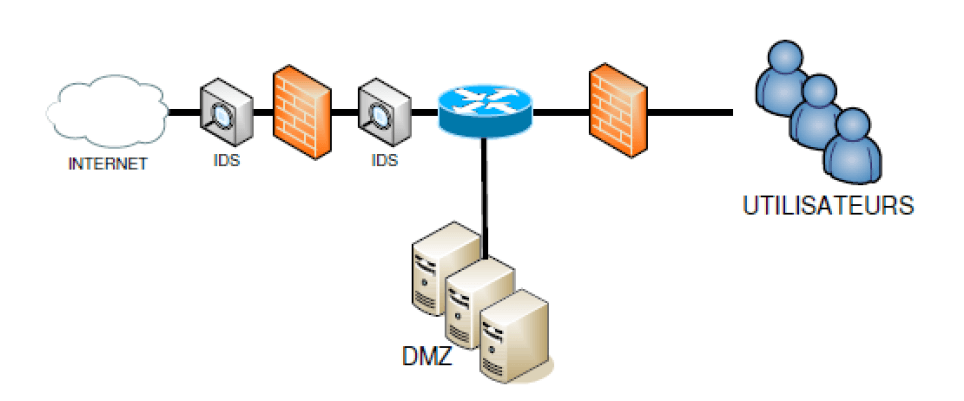
\includegraphics[width=1\textwidth]{assets/reseau.png}
    \caption[Exemple de disposition de sonde IDS dans le réseau d'un OIV (source:\href{https://blogger.googleusercontent.com/img/b/R29vZ2xl/AVvXsEhz0rffx8tqoJRqjF0Hf3LAERS8e7tpmQVnPzlBITzud8iMUOh63zfDIyLKLXnQprLLNAycblYb02W3Y4004q3ruHhdZ3T9Dy7KTMyydsLMRjR2UGkzQ6hIOcwM8DiSLeLp0pZeyyCt5CDl/s1600/Capture.PNG}{eventus-networks.blogspot.com})]{Exemple de disposition de sonde IDS dans le réseau d'un OIV}\label{fig:test}
\end{figure}

\vspace{1em}

Ces règles sont créées à partir d'indicateurs de compromission (IOC) établis en interne ou grâce à des renseignements externes provenant de CERT partenaires (comme le CERT-FR de l'ANSSI) ou d'agences privées de cyber-renseignement (également appelées CTI). Les règles générées par ces partenaires externes posent souvent des problèmes :\\

\begin{itemize}[itemsep=0.75em]
    \item[•] Les règles générées sont fréquemment génériques et mal adaptées, engendrant trop d'événements inutiles ou redondants dans le réseau où elles sont mises en œuvre (ces réseaux sont tous basés sur des technologies différentes).
    \item[•] Les renseignements extérieurs ne proviennent que d'une poignée d'acteurs, et l'agence ne peut être certaine de pouvoir détecter toutes les menaces existantes à l'état de l'art.\\
\end{itemize}

\newpage

Ces difficultés de l'AMSN sont communes aux institutions publiques et aux entreprises qui doivent remplir les mêmes missions. Cela légitime la problématique posée : "Comment mettre en place un outil automatisé de génération de règles de détection d’intrusion ?"\\

Pour aborder cette problématique, il faut se poser les questions suivantes :
\vspace{0.5em}
\begin{itemize}[itemsep=0.5em]
    \item[•] Où recueillir le cyber-renseignement nécessaire à l'établissement des IOC ? Et comment évaluer la qualité de ces renseignements ?
    \item[•] Comment générer des règles automatiquement à partir de ces IOC ?
    \item[•] Comment s'assurer que ces règles soient aussi pertinentes que possible pour la partie prenante supervisée ?\\
\end{itemize}

Mes travaux, menés dans le cadre de l'AMSN, visent à répondre à cette problématique et à fournir une solution capable de résoudre les problèmes posés à l'Agence ou à tout autre acteur similaire oeuvrant pour la protection des systèmes d'information.
}

\newpage

\section{Organisation du stage}
\label{chap1:section3}
{\fontsize{14pt}{16pt}\selectfont
    %%%%%%%%%%%%%%%%%%%%%%%%%%%%
% SECTION                  %
%%%%%%%%%%%%%%%%%%%%%%%%%%%%
\vspace{1em}

Le stage s'est déroulé du 1er avril au 30 septembre 2024. Pendant cette période, j'ai bénéficié d'un bureau au sein du SOC-MC avec un ordinateur personnel connecté à un réseau séparé sur lequel j'ai été libre de réaliser tous les développements nécessaires à la réalisation de mon projet. Cette configuration avait l'avantage de me permettre d'être proche des personnes impliquées dans l'outil sur lequel je travaillais, ainsi tout au long de mon stage j'ai pu disposer de l'expérience et des conseils, d'une part, des analystes SOC de l'AMSN et, d'autre part, de mon tuteur de stage Bruno VALENTIN, qui m'a partagé les connaissances et les avis du CSIRT.\\

Le stage s’est déroulé en trois parties distinctes :
\vspace{0.5em}
\begin{enumerate}[itemsep=0.5em]
    \item Apprentissage des technologies et du contexte
    \item Développement de la solution
    \item Rédaction de la thèse\\
\end{enumerate}

La première partie correspond à mon premier mois de stage, au cours duquel j'ai pris connaissance de mon environnement de travail et des missions de l'Agence, ainsi que des différents corps qui la composent. Au cours des semaines inaugurales de mon stage, j'ai dédié le plus clair de mon temps à suivre le travail quotidien de mes collègues pour appréhender les outils qu'ils utilisaient et comprendre comment ils fonctionnaient.\\

Après cette phase d'apprentissage, j'ai pu commencer à développer la solution relative à 
la problématique visée. Cette phase a duré quatre mois, à l'issue desquels j'ai soumis la solution et la documentation à mon tuteur. Mon tuteur s'est chargé quant à lui de la mise en production de mon travail pendant le mois qui a suivi.\\

Le dernier mois de stage et jusqu'à son terme, ayant finalisé la mission qui m'avait été confiée par mon tuteur, j'ai pu me concentrer avec son appui à parfaire, au sein de l'agence, la rédaction de la présente thèse, en l'étoffant par des échanges constructifs.\\

Tout au long de ces périodes, Bruno VALENTIN et Sébastien ABBONDANZA ont suivi mon travail en programmant des rapports bimensuels au cours desquels j'ai régulièrement fait état de mes progrès et reçu des conseils de leur part.
}

%L'ajout d'une url~\url{www.google.fr}\\
%L'ajout d'une référence~\cite{web001}\\
%Ajout d'une image~\ref{fig:test}\\

%  \begin{figure}[h]%
%    \center%
%    \includegraphics[width=0.3\textwidth]{assets/logonoir.png}
%    \caption[Image de réference]{Test Image}\label{fig:test}
%  \end{figure}


%\begin{table}\begin{center}
%\begin{tabular}{c|c}
%Entrée & Sortie \\ \hline
%A & B \\
%C & D
%\end{tabular}
%\caption{Test Table}\end{center}
%\end{table}

%This is a second subsection\cite{gen1972}, \cite{schaeffer99}. ~\\

%   \begin{description}\addtolength{\itemsep}{-0.35\baselineskip}%
%     \item[\textbullet~\bfseries Menu Item] \hfill \\%
%       Menu Description.~\\%
%       {\textbf{Focus topics:~}\emph{Topic one, topic two, topic three, ...}}%
%     %
%     \item[\textbullet~\bfseries Menu Item] \hfill \\%
%       Menu Description.~\\%
%       {\textbf{Focus topics:~}\emph{Topic one, topic two, topic three, ...}}%
%     %
%     \item[\textbullet~\bfseries Menu Item] \hfill \\%
%       Menu Description.~\\%
%       {\textbf{Focus topics:~}\emph{Topic one, topic two, topic three, ...}}%
%   \end{description}

%   Also bullets such as:%
%   \begin{itemize}\addtolength{\itemsep}{-0.35\baselineskip}%
%     \item One%
%     \item Two%
%     \item Three%
%     \item Four%
%     \item \ldots%
%   \end{itemize}%
%   %

% \begin{equation} \label{eq:1}
% \sum_{i=0}^{\infty} a_i x^i
% \end{equation}

% The equation \ref{eq:1} is a typical power series.

\chapter{Définition du sujet}%
\label{chap:2}
%%%%%%%%%%%%%%%%%%%%%%%%%%%%
% CHAPTER                  %
%%%%%%%%%%%%%%%%%%%%%%%%%%%%

\section{L’enjeu de la détection des menaces}
\label{chap2:section1}
{\fontsize{14pt}{16pt}\selectfont
    %%%%%%%%%%%%%%%%%%%%%%%%%%%%
% SECTION                  %
%%%%%%%%%%%%%%%%%%%%%%%%%%%%
\vspace{0.75em}

Les cyberattaques représentent l'une des menaces les plus sérieuses pour les institutions publiques et les entreprises privées. Les attaquants, qu'il s'agisse de pirates informatiques ayant des objectifs malveillants ou d'agents étatiques, utilisent des méthodes de plus en plus sophistiquées pour s'infiltrer dans les systèmes, voler des données sensibles, perturber les opérations et causer des dommages financiers et/ou des atteintes à la réputation. \hyperref[biblio]{[8]}\\

Ces acteurs malveillants poursuivent l’amélioration constante de leurs capacités à des fins de gain financier, d’espionnage ou encore de déstabilisation. Cette amélioration s’illustre en particulier dans le ciblage des  attaquants qui cherchent à obtenir des accès discrets et pérennes aux réseaux de leurs victimes. Les acteurs malveillants tentent de compromettre des équipements périphériques qui  leur offrent un accès plus furtif et persistant. Ce ciblage périphérique se transpose également dans le type d’entités attaquées et confirme l’intérêt des attaquants pour les prestataires, les fournisseurs, les sous-traitants, les organismes de tutelle et l’écosystème plus large de leurs cibles finales.\\

Cette amélioration continue des stratégies et des compétences des attaquants met en évidence les limites de la sécurité des réseaux. La mise en place d'architectures sécurisées (pare-feu, antivirus, réseaux locaux virtuels, etc.) ne garantit pas qu'une intrusion informatique soit impossible. Face à des attaquants suffisamment motivés, une erreur humaine ou une vulnérabilité encore inconnue (dite Zero-Day) finira par permettre une intrusion sur le réseau défendu ou sur celui d'un partenaire dont le réseau dépend, quelle que soit la qualité de la sécurité mise en place.\\

Cette faiblesse intrinsèque de la sécurité informatique rend obligatoire la mise en place, au sein des infrastructures numériques sécurisées, d'outils capables de gérer la possibilité que l'infrastructure défendue soit déjà compromise. C'est le rôle que jouent les systèmes de détection d'intrusion en permettant la détection des tentatives d'intrusion au sein d'un réseau supervisé. \hyperref[biblio]{[5]}
}

\newpage

\section{Les systèmes de détection d’intrusion}
\label{chap2:section2}
{\fontsize{14pt}{16pt}\selectfont
    %%%%%%%%%%%%%%%%%%%%%%%%%%%%
% SECTION                  %
%%%%%%%%%%%%%%%%%%%%%%%%%%%%
\vspace{1em}

La détection des intrusions consiste à surveiller les événements qui se produisent dans un système ou un réseau informatique et à les analyser pour y déceler des signes d'intrusion, définis comme des tentatives pour compromettre la confidentialité, l'intégrité, la disponibilité ou pour contourner les mécanismes de sécurité d'un ordinateur ou d'un réseau.\\

Les intrusions sont causées par des attaquants qui accèdent aux systèmes depuis l'internet, par des utilisateurs autorisés des systèmes qui tentent d'obtenir des privilèges supplémentaires pour lesquels ils ne sont pas autorisés, et par des utilisateurs autorisés qui abusent des privilèges qui leur sont accordés. Les systèmes de détection d'intrusion (IDS) sont des produits logiciels ou matériels qui automatisent ce processus de surveillance et d'analyse.\\ 

Un IDS peut être configuré pour surveiller différents types de trafic, tels que les paquets de données, les connexions réseau, les logs de systèmes, etc. Lorsqu'il détecte une activité suspecte, l'IDS génère une alerte qui est envoyée, permettant de prendre des mesures pour bloquer l'attaque ou corriger la vulnérabilité. \hyperref[biblio]{[3]}\\

\vspace{1em}

\subsection{Types d'IDS }

\vspace{1em}

La façon la plus courante de classer les IDS est de les regrouper par source d'information. Certains IDS analysent les paquets du réseau, capturés à partir des flux passants au sein du réseau pour trouver les attaquants. D'autres IDS analysent les sources d'information générées par les systèmes d'exploitation ou les logiciels d'application présents sur les postes utilisateurs pour y trouver des signes d'intrusion. \hyperref[biblio]{[6 - 7]}

\vspace{1em}

\subsubsection{Les systèmes de détection d'intrusion réseau}

\vspace{0.5em}

La majorité des systèmes commerciaux de détection d'intrusion sont basés sur les réseaux. Ces systèmes de détection d'intrusion réseau (ou NIDS : Network Intrusion Detection System) détectent les attaques en capturant et en analysant les paquets du réseau. À l'écoute d'un segment de réseau ou d'un commutateur, un système de détection d'intrusion en réseau peut surveiller le trafic réseau affectant plusieurs hôtes connectés au segment de réseau.\\

\newpage

\begin{figure}[h]%
    \center%
    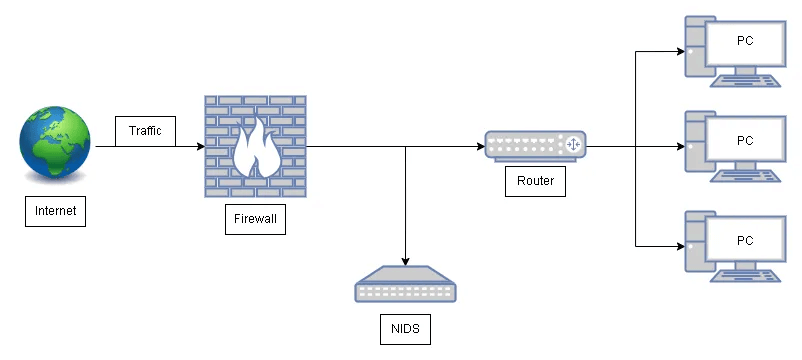
\includegraphics[width=0.9\textwidth]{assets/NIDS.png}
    \caption[Exemple de systèmes de détection d'intrusion réseau (NIDS) (source: \href{https://miro.medium.com/v2/resize:fit:4800/format:webp/1*Jbw1iMzBztCaUokJnqePBg.png}{techno-skills.com})]{Exemple de systèmes de détection d'intrusion réseau (NIDS)}\label{fig:NIDSexemple}
\end{figure}

\vspace{1em}

\textit{Avantages des IDS en réseau :}\\

\begin{itemize}[itemsep=1em]
    \item[•] Quelques IDS bien placés peuvent surveiller un grand réseau ;
    \item[•] Le déploiement d'IDS en réseau a peu d'impact sur un réseau existant. Les IDS basés sur le réseau sont généralement des dispositifs passifs qui écoutent sur un fil de réseaux sans interférer avec le fonctionnement normal d'un réseau ;
    \item[•] Les IDS en réseau peuvent être configurés de manière à être hautement sécurisés contre les attaques et très difficiles à détecter pour les attaquants.\\
\end{itemize}

\vspace{1em}

\textit{Inconvénients des IDS en réseau :}\\

\begin{itemize}[itemsep=1em]
    \item[•] Les IDS basés sur le réseau peuvent avoir des difficultés à traiter tous les paquets dans un réseau important ou très fréquenté et, par conséquent, ne pas reconnaître une attaque lancée pendant les périodes de fort trafic ;
    \item[•] Les IDS basés sur le réseau ne peuvent pas analyser les informations chiffrées. Ce problème s'aggrave car de plus en plus d'organisations (et d'attaquants) utilisent des réseaux privés virtuels ;
    \newpage
    \item[•] La plupart des IDS basés sur le réseau ne peuvent pas déterminer si une attaque a réussi ou non ; ils peuvent seulement discerner qu'une attaque a été initiée. Cela signifie qu'après la détection d'une attaque par un système IDS basé sur le réseau, un examen manuel (ou une corrélation automatique à l'aide d'autres sources de données comme des logs) devra être effectué afin de caractériser si l'attaque a été réussie.
\end{itemize}

\vspace{1em}

\subsubsection{Systèmes de détection d'intrusion au niveau de l'hôte}

\vspace{0.5em}

Les systèmes de détection d'intrusion au niveau de l'hôte (ou HIDS : Host-based Intrusion Detection System), reposant sur l'hôte, fonctionnent sur la base des informations collectées à l'intérieur des appareils des utilisateurs. Les IDS basés sur l'hôte utilisent normalement des sources d'information de deux types : les pistes d'audit du système d'exploitation et les journaux du système. Ils permettent également de prendre un instantané des fichiers système existants et de les comparer à l'instantané précédant pour générer des alertes en cas de modifications.\\

\vspace{1em}

\begin{figure}[h]%
    \center%
    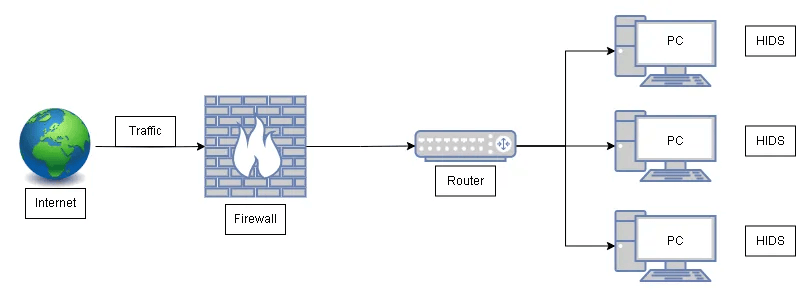
\includegraphics[width=0.9\textwidth]{assets/HIDS.png}
    \caption[Exemple de systèmes de détection d'intrusion au niveau de l'hôte (HIDS) (source: \href{https://miro.medium.com/v2/resize:fit:4800/format:webp/1*Jbw1iMzBztCaUokJnqePBg.png}{techno-skills.com})]{Exemple de systèmes de détection d'intrusion au niveau de l'hôte (HIDS)}\label{fig:HIDSexemple}
\end{figure}

\vspace{1em}

\textit{Avantages des IDS basés sur les hôtes :}\\

\begin{itemize}[itemsep=1em]
    \item[•] Les IDS basés sur l'hôte, grâce à leur capacité à surveiller les événements locaux d'un hôte, peuvent détecter des attaques qui ne peuvent l'être par un IDS basé sur le réseau ;

\newpage

    \item[•] Les IDS basés sur l'hôte peuvent fonctionner dans un environnement où le trafic réseau est chiffré, les sources d'information étant générées avant le chiffrement des données et/ou après le déchiffrement des données sur l'hôte de destination ;
    \item[•] Les IDS basés sur l'hôte ne sont pas affectés par les réseaux commutés.\\
\end{itemize}

\vspace{1em}

\textit{Inconvénients des IDS basés sur les hôtes :}\\
\vspace{0.5em}
\begin{itemize}[itemsep=1em]
    \item[•] Les IDS basés sur l'hôte sont plus difficiles à gérer, car les informations doivent être configurées et gérées pour chaque hôte surveillé ;
    \item[•] Étant donné que les sources d'information des IDS basés sur l'hôte résident sur l'hôte ciblé par les attaques, l'IDS peut être attaqué et désactivé dans le cadre de l'attaque ;
    \item[•] Les IDS basés sur l'hôte ne sont pas bien adaptés à la détection des scans de réseau ou d'autres formes de surveillance ciblant l'ensemble d'un réseau, car l'IDS ne voit que les paquets de réseau reçus par son hôte.
\end{itemize}

\newpage

\subsection{Méthode de détection }

\vspace{1em}

Les technologies IDS utilisent de nombreuses méthodologies pour détecter les incidents. Ces méthodologies peuvent être regroupées en deux grandes catégories : celles basées sur les signatures et celles basées sur les anomalies.  La plupart des technologies IDS utilisent plusieurs méthodologies de détection, séparément ou intégrées, afin de fournir une détection plus large et plus précise. \hyperref[biblio]{[1]}

\subsubsection{Les IDS à base de signatures}
\label{chap2:IDSsignature}

\vspace{0.5em}

Les IDS à base de signatures ont une base de données comportant un ensemble de signatures d’attaques (base de signatures). Le principe de fonctionnement est le test de correspondance. Les données du réseau sont analysées et comparées aux signatures d’attaques connues stockées dans la base de signatures. En cas de correspondance, une alerte est émise. Un avantage de ce système est qu’il a une meilleure précision lorsque les règles de signature sont correctes. Cette base de signatures est en général pré-initialisée avec des données de l’éditeur de l’IDS et mise à jour régulièrement pour prendre en compte les nouvelles attaques.\\

La détection basée sur les signatures est très efficace pour détecter les menaces connues, mais largement inefficace pour détecter les menaces inconnues. Elle a l'avantage d'être facile à mettre en place, mais sa principale limite est que si l'attaquant est conscient des règles de détection en place, il peut modifier légèrement sa technique pour qu'elle ne soit plus détectable.\\

\begin{figure}[h]%
    \center%
    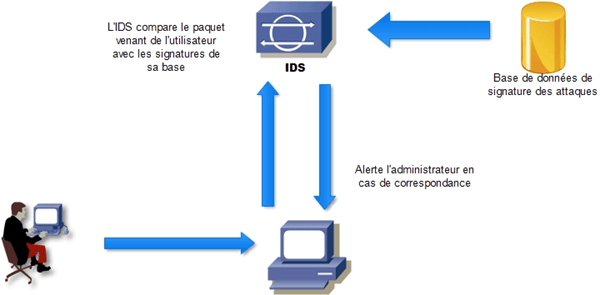
\includegraphics[width=0.9\textwidth]{assets/IDSbaseSignatures.png}
    \caption[Procédure de détection d’attaques d’un IDS à base de signatures (source: \href{https://techno-skills.com/wp-content/uploads/2020/12/image-4.png}{techno-skills.com})]{Procédure de détection d’attaques d’un IDS à base de signature}\label{fig:ids-signature}
\end{figure}

\newpage

\subsubsection{Les IDS à base d’anomalies}

\vspace{0.5em}

Cette catégorie d’IDS utilise un modèle statistique du fonctionnement de référence du réseau qui peut comprendre la bande passante utilisée, les protocoles définis pour le trafic, les ports et les périphériques qui font partie du réseau. Il surveille régulièrement le trafic réseau et le compare au modèle statistique. En cas d’anomalie ou de divergence, l’administrateur est alerté. Un avantage de ce système est qu’il peut détecter des attaques nouvelles dont le comportement s’éloigne suffisamment de la normale.\\

Malheureusement, les détecteurs d'anomalies et les systèmes de détection d'intrusion qui en découlent produisent souvent un grand nombre de fausses alertes, car les modèles normaux de comportement des utilisateurs et des systèmes peuvent varier considérablement sans être prévisibles. Ce type de détection est difficile à utiliser de manière efficace.\\

\begin{figure}[h]%
    \center%
    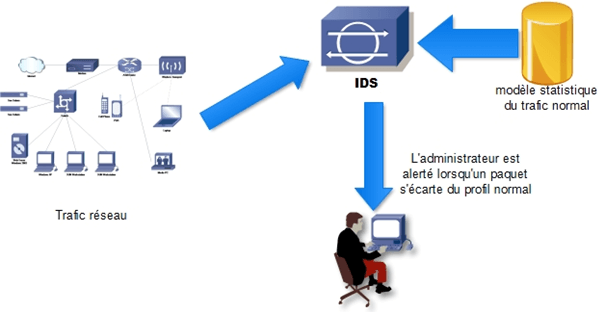
\includegraphics[width=0.9\textwidth]{assets/IDSbaseAnomalies.png}
    \caption[Procédure de détection d’attaques d’un IDS à base d’anomalies (source: \href{https://techno-skills.com/wp-content/uploads/2020/12/image-5.png}{techno-skills.com})]{Procédure de détection d’attaques d’un IDS à base d’anomalies}\label{fig:ids-anomalie}
\end{figure}

\subsubsection{\textit{Note}}
Dans le cadre de mes travaux, j'ai travaillé avec des systèmes de détection d'intrusion réseaux faisant de la détection par signatures. Ce choix technologique se justifie dans le contexte de l'AMSN par le besoin de posséder une capacité de détection pouvant fonctionner sur les réseaux de tous les OIV en même temps sans perturber leurs activités usuelles. L'utilisation de la détection à base d’anomalies et des Systèmes de détection d’intrusion au niveau de l’hôte serait beaucoup plus difficile par la diversité des OIV et demanderait un niveau de connaissance sur les réseaux supervisés que l'Agence n'a pas vocation à connaître.
}

\newpage

\section{Les indicateurs de compromission}
\label{chap2:section3}
{\fontsize{14pt}{16pt}\selectfont
    %%%%%%%%%%%%%%%%%%%%%%%%%%%%
% SECTION                  %
%%%%%%%%%%%%%%%%%%%%%%%%%%%%
\vspace{1em}

Les IDS, notamment ceux faisant de la détection par signatures, ont besoin d'une base de référentiels pour savoir quoi détecter. C'est ce rôle que jouent les indicateurs de compromission (ou IOC : Indicator Of Compromise)\\

Un indicateur de compromission, en sécurité informatique, est une déviance ou un artéfact observé sur un réseau ou dans un système d'exploitation qui indique, avec un niveau de certitude déterminé, une intrusion informatique. Des indicateurs de compromission peuvent être : des signatures virales, des adresses IP particulières, des hachages de fichiers malveillants, des URLs ou des noms de domaine de serveurs de commande et de contrôle de botnets, etc. \hyperref[biblio]{[4]}\\

\begin{figure}[h]%
    \center%
    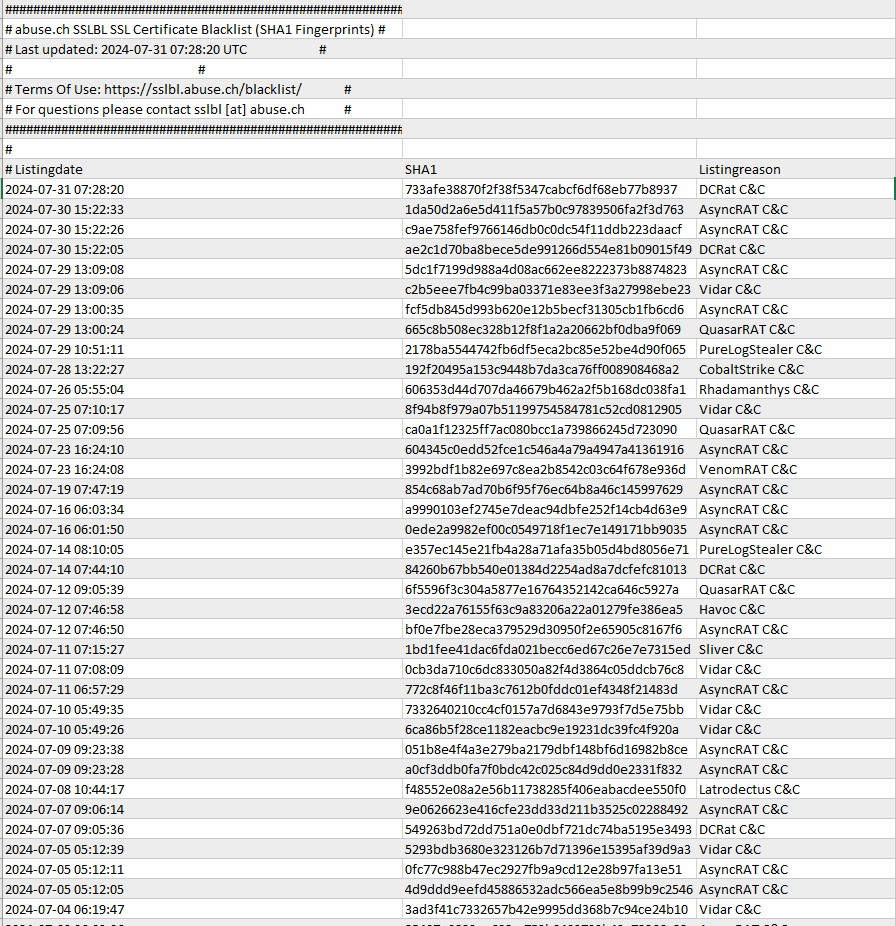
\includegraphics[width=0.74\textwidth]{assets/IOC.png}
    \caption[Exemple de liste d'IOC de hachages de fichiers malveillants fournie par \textit{abuse.ch} (source: \href{https://sslbl.abuse.ch/blacklist/sslblacklist.csv}{sslbl.abuse.ch/blacklist/sslblacklist.csv})]{Exemple de liste d'IOC de hachages de fichiers malveillants fournie par \textit{abuse.ch}}\label{fig:ioc}
\end{figure}

\newpage

Ces IOC sont découverts à la suite d'investigations numériques (également appelées renseignements sur les menaces ou \textit{threat intelligence}) menées sur les traces laissées par des acteurs malveillants en ligne ou à partir d'une analyse post-incident des techniques utilisées par les attaquants qui ont tenté ou réussi à pénétrer dans le système informatique. Ces IOC sont ensuite partagés par différents acteurs:\\

\begin{itemize}[itemsep=1em]
    \item[•] \textbf{Organismes de cybersécurité}\\
    La plupart des CERT étatiques (CERT-FR Français, US-CERT Américains, etc.) ou privés (CERT Orange, CERT Crédit Agricole, etc.) réalisent en partie eux-mêmes de la collecte d'IOC qu'ils partagent en privé entre agences lorsque des accords de collaboration existent, mais aussi publiquement pour une part\footnote{Exemple source publique du CERT-FR: \url{https://www.cert.ssi.gouv.fr/ioc/}}.
    \item[•] \textbf{Entreprises spécialisées de CTI}\\
    Le besoin de renseignement sur les menaces existantes ne cessant de croître, des sociétés spécialisées se sont créées pour répondre à cette demande (CrowdStrike, Sekoia.io, etc.) en plus des autres services de cybersécurité qu'elles peuvent pourvoir. En échange d'un contrat rémunéré, ces sociétés fournissent des listes d'IOC régulièrement mises à jour.
    \item[•] \textbf{Plate-formes d'échange libre de renseignement cyber}\\
    Pour faire face à l'ampleur des menaces, des plateformes de coopération CTI ont commencé à apparaître en ligne, impliquant des organisations étatiques et privées ainsi que des professionnels individuels du secteur. Grâce à ces plateformes (MISP, alienvault, threatfox, etc.), les utilisateurs peuvent s'alerter mutuellement des évènements cyber en cours et partager les IOC qu'ils possèdent.
\end{itemize}
}

% \begin{itemize}
% 	\item The individual \index{Entries}{entries} are indicated with a black dot, a so-called bullet.
% Tout au long de ces périodes, Bruno VALENTIN et Sébastien ABBONDANZA ont suivi mon travail en programmant des rapports bimensuels au cours desquels j'ai régulièrement fait part de mes progrès et reçu des conseils de leur part.\\
% 	\item The text in the entries may be of any length.
% \end{itemize}

% \begin{theorem}\label{theo1}
% Soit $n$ un entier naturel. Si $n$ est premier alors il n'est divisible que par 1 et par lui-même.
% \end{theorem}

% \begin{proof}
% Here is my proof.
% \end{proof}

% \begin{definition}\label{def1}
% Soit $A$ une courbe...
% \end{definition}

% Ici, il s'agit de l'utilisation de TB %\nomenclature[TB]{TB}{Très Bien} qui consiste à parler Très Bien. 
% \gls{abc} et \gls{efg} sont des acronyms et des abbréviations... La méthode \gls{svm} est également couramment utilisée.

% \begin{exemple}\label{exo1}
% On considère le cas particulier... 
% \end{exemple}

\chapter{Réalisation de la solution}%
\label{chap:3}
%%%%%%%%%%%%%%%%%%%%%%%%%%%%
% CHAPTER                  %
%%%%%%%%%%%%%%%%%%%%%%%%%%%%
\label{chap3:intro}
{\fontsize{14pt}{16pt}\selectfont
    %%%%%%%%%%%%%%%%%%%%%%%%%%%%
% Intro chapter            %
%%%%%%%%%%%%%%%%%%%%%%%%%%%%

Comme énoncé dans la section \hyperref[chap1:section2]{\textit{\textbf{Problématique}}}, l'AMSN dispose déjà de sondes installées à des points clés des réseaux des OIV. Il s'agit de sondes qualifiées par l'ANSSI et délivrées par une société spécialisée qui fournit également un logiciel permettant d'envoyer directement des règles Suricata aux sondes. Les règles de détection des sondes sont quant à elles mises à jour quotidiennement afin de rester opérationnelles face à l'état de l'art connu de la menace. \\

 Le processus de gestion des sondes préexistant au sein de l'Agence, lorsque j'ai commencé à travailler, était le suivant :\\

\begin{figure}[h]%
    \center%
    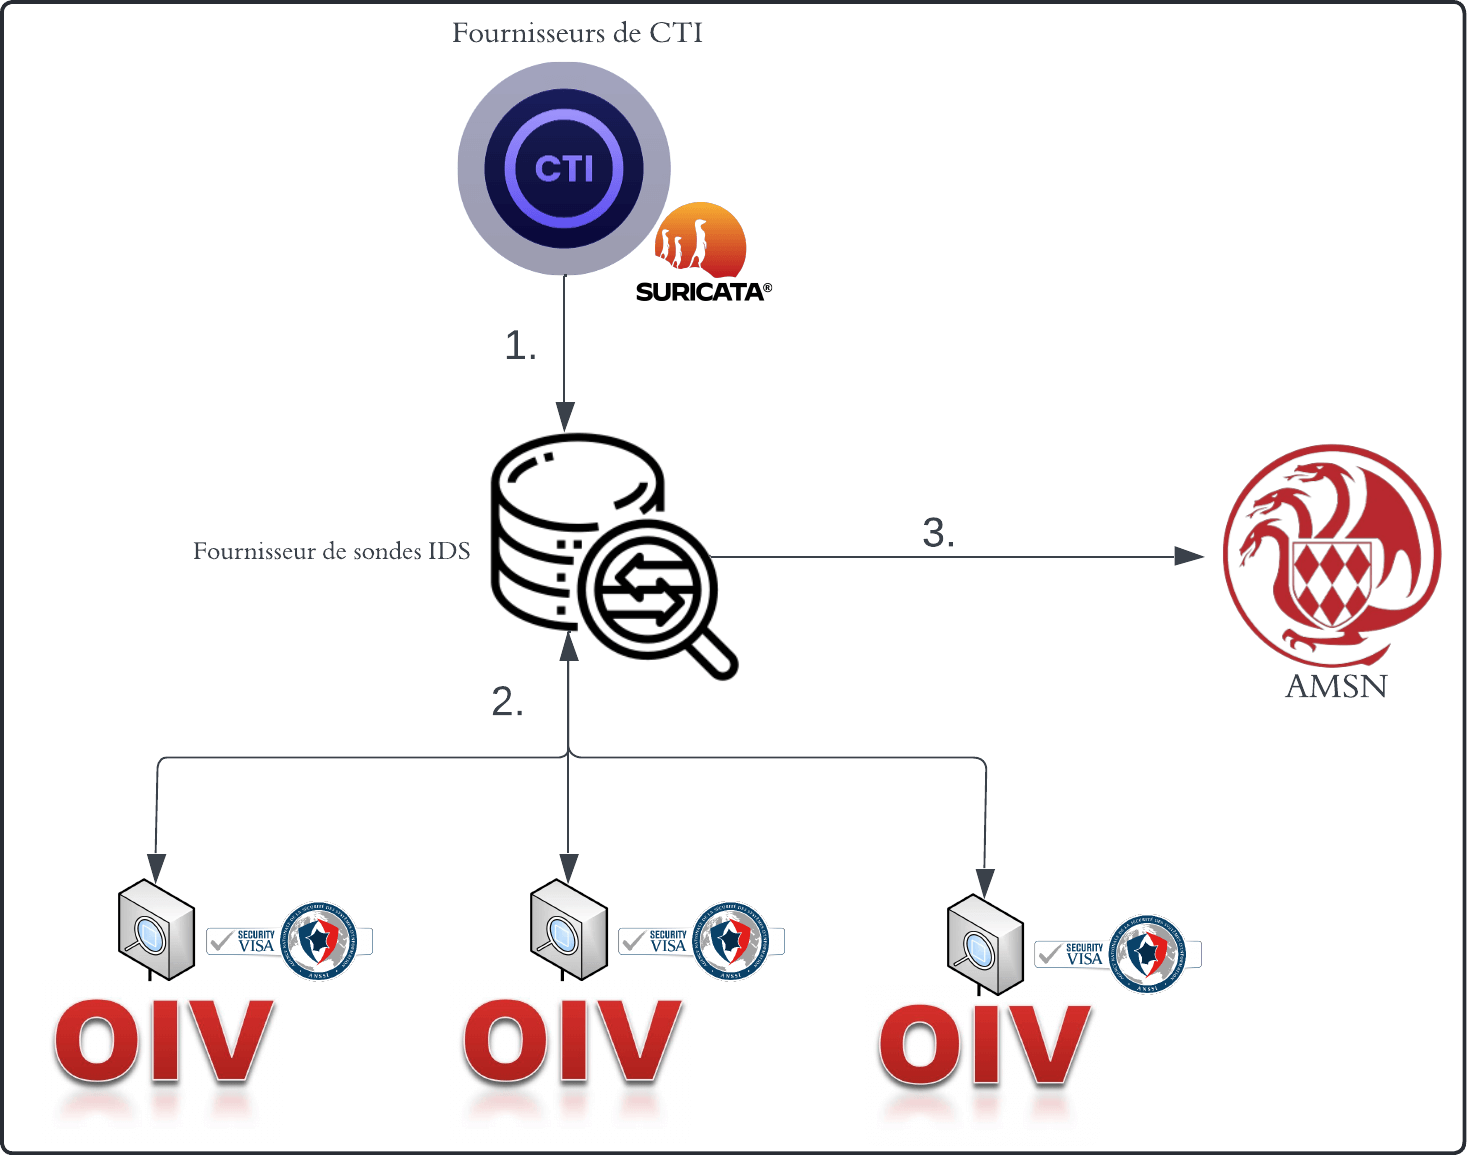
\includegraphics[width=0.73\textwidth]{assets/shemaProcessAMSN.png}
    \caption[Processus d'alimentation des sondes]{Processus d'alimentation des sondes}\label{fig:shemaProcessAMSN}
\end{figure}

\newpage

\begin{enumerate}[itemsep=1em]
    \item L'agence recoit, de la part de partenaires, de la CTI sous la forme de règles Suricata exploitables ;
    \item Les règles sont envoyées au système de gestion des sondes fourni par l'entreprise partenaire spécialisée, qui les distribue aux sondes des OIV ;
    \item Les alertes générées par les sondes sont remontées jusqu'au SOC-MC de l'AMSN.\\
\end{enumerate}

Mon projet professionnel n'a pas profondément modifié ce processus, mais l'a amélioré en s'interposant entre les fournisseurs de CTI et le système de gestion des sondes afin d'améliorer la qualité des règles de détection arrivant finalement dans les sondes IDS.\\

Ce travail d'amélioration s'est organisé en trois grandes étapes :\\

\begin{enumerate}[itemsep=1em]
    \item Création d'un programme automatisé pour contrôler la qualité des règles fournies par les partenaires afin de les filtrer et de les formater avant de les envoyer aux sondes des OIV ;
    \item Mise en place et exploitation d'une instance locale de MISP pour enrichir le programme avec de nouvelles sources de renseignement ;
    \item Exploitation des travaux précédents pour adapter automatiquement les règles envoyées en fonction de l'OIV cible.\\
\end{enumerate}

J'ai réalisé ces différentes missions en suivant la même méthodologie. Tout d'abord, une phase de réflexion était menée conjointement avec mon tuteur de stage et le responsable du SOC-MC pour identifier les attendus du travail à produire. Puis, une phase de développement et de test s'ensuivait pour correspondre à ces attentes. Pour conclure par une phase de rédaction de documentation et de mise en place de tests unitaires afin de permettre la continuité de mon travail sur le temps et sa potentielle prise en main par d'autres personnes.
}

\newpage

\section{Génération de règles normées}
\label{chap3:section1}
{\fontsize{14pt}{16pt}\selectfont
    %%%%%%%%%%%%%%%%%%%%%%%%%%%%
% SECTION                  %
%%%%%%%%%%%%%%%%%%%%%%%%%%%%
\vspace{1em}
Le premier mois de mon stage, passé en immersion au sein de l'Agence et aux côtés des membres du SOC-MC, m'a permis d'observer et de comprendre le fonctionnement et l'enjeu des données ainsi que des systèmes sur lesquels j'allais travailler. A la suite des recommandations des analystes du SOC-MC et autres entretiens avec Bruno VALENTIN et Sébastien ABBONDANZA, un premier cahier des charges des besoins a été établi. Cette documentation a servi de base au développement d'un outil qui contribuera à améliorer le processus actuel de mise à jour des règles en répondant aux besoins définis ci-après :\\

\begin{itemize}[itemsep=1em]
    \item[•] L'outil doit être capable de récupérer et de centraliser toutes les règles, quelle que soit leur source (partenaires de CTI ou internes) ;
    \item[•] L'outil doit vérifier la conformité des règles récupérées avec les sondes utilisées et supprimer toute règle dupliquée ;
    \item[•] L'outil devra créer des fichiers de règles portant un nom unique pour chaque sonde ;
    \item[•] L'outil permettra aux analystes du SOC-MC de spécifier des règles à modifier ou à supprimer avant de les envoyer aux sondes ;
    \item[•] L'outil devra rendre compte des résultats du programme.\\
\end{itemize}

L'objectif de cet outil est de répondre à une partie des problèmes énoncés dans ma problématique et à ceux de l'Agence. Le choix technologique de développement de l'outil s'est porté sur le langage de programmation python. L'outil aurait pu être développé à l'aide d'autres technologies, mais Python a été choisi pour la facilité d'utilisation qu'il offre dans la production de scripts facilement exportables. De plus, ce langage me fut suggéré car il est également maîtrisé par la majorité de mes collègues au sein de l'AMSN, ce qui permet à mon travail d'être facilement relu et repris par d'autres personnes au sein de l'Agence.\\

\newpage

Le diagramme de flux de l'outil développé, qui sera analysé en détail dans la suite de mon argumentaire, est le suivant :\\

\begin{figure}[h]%
    \center%
    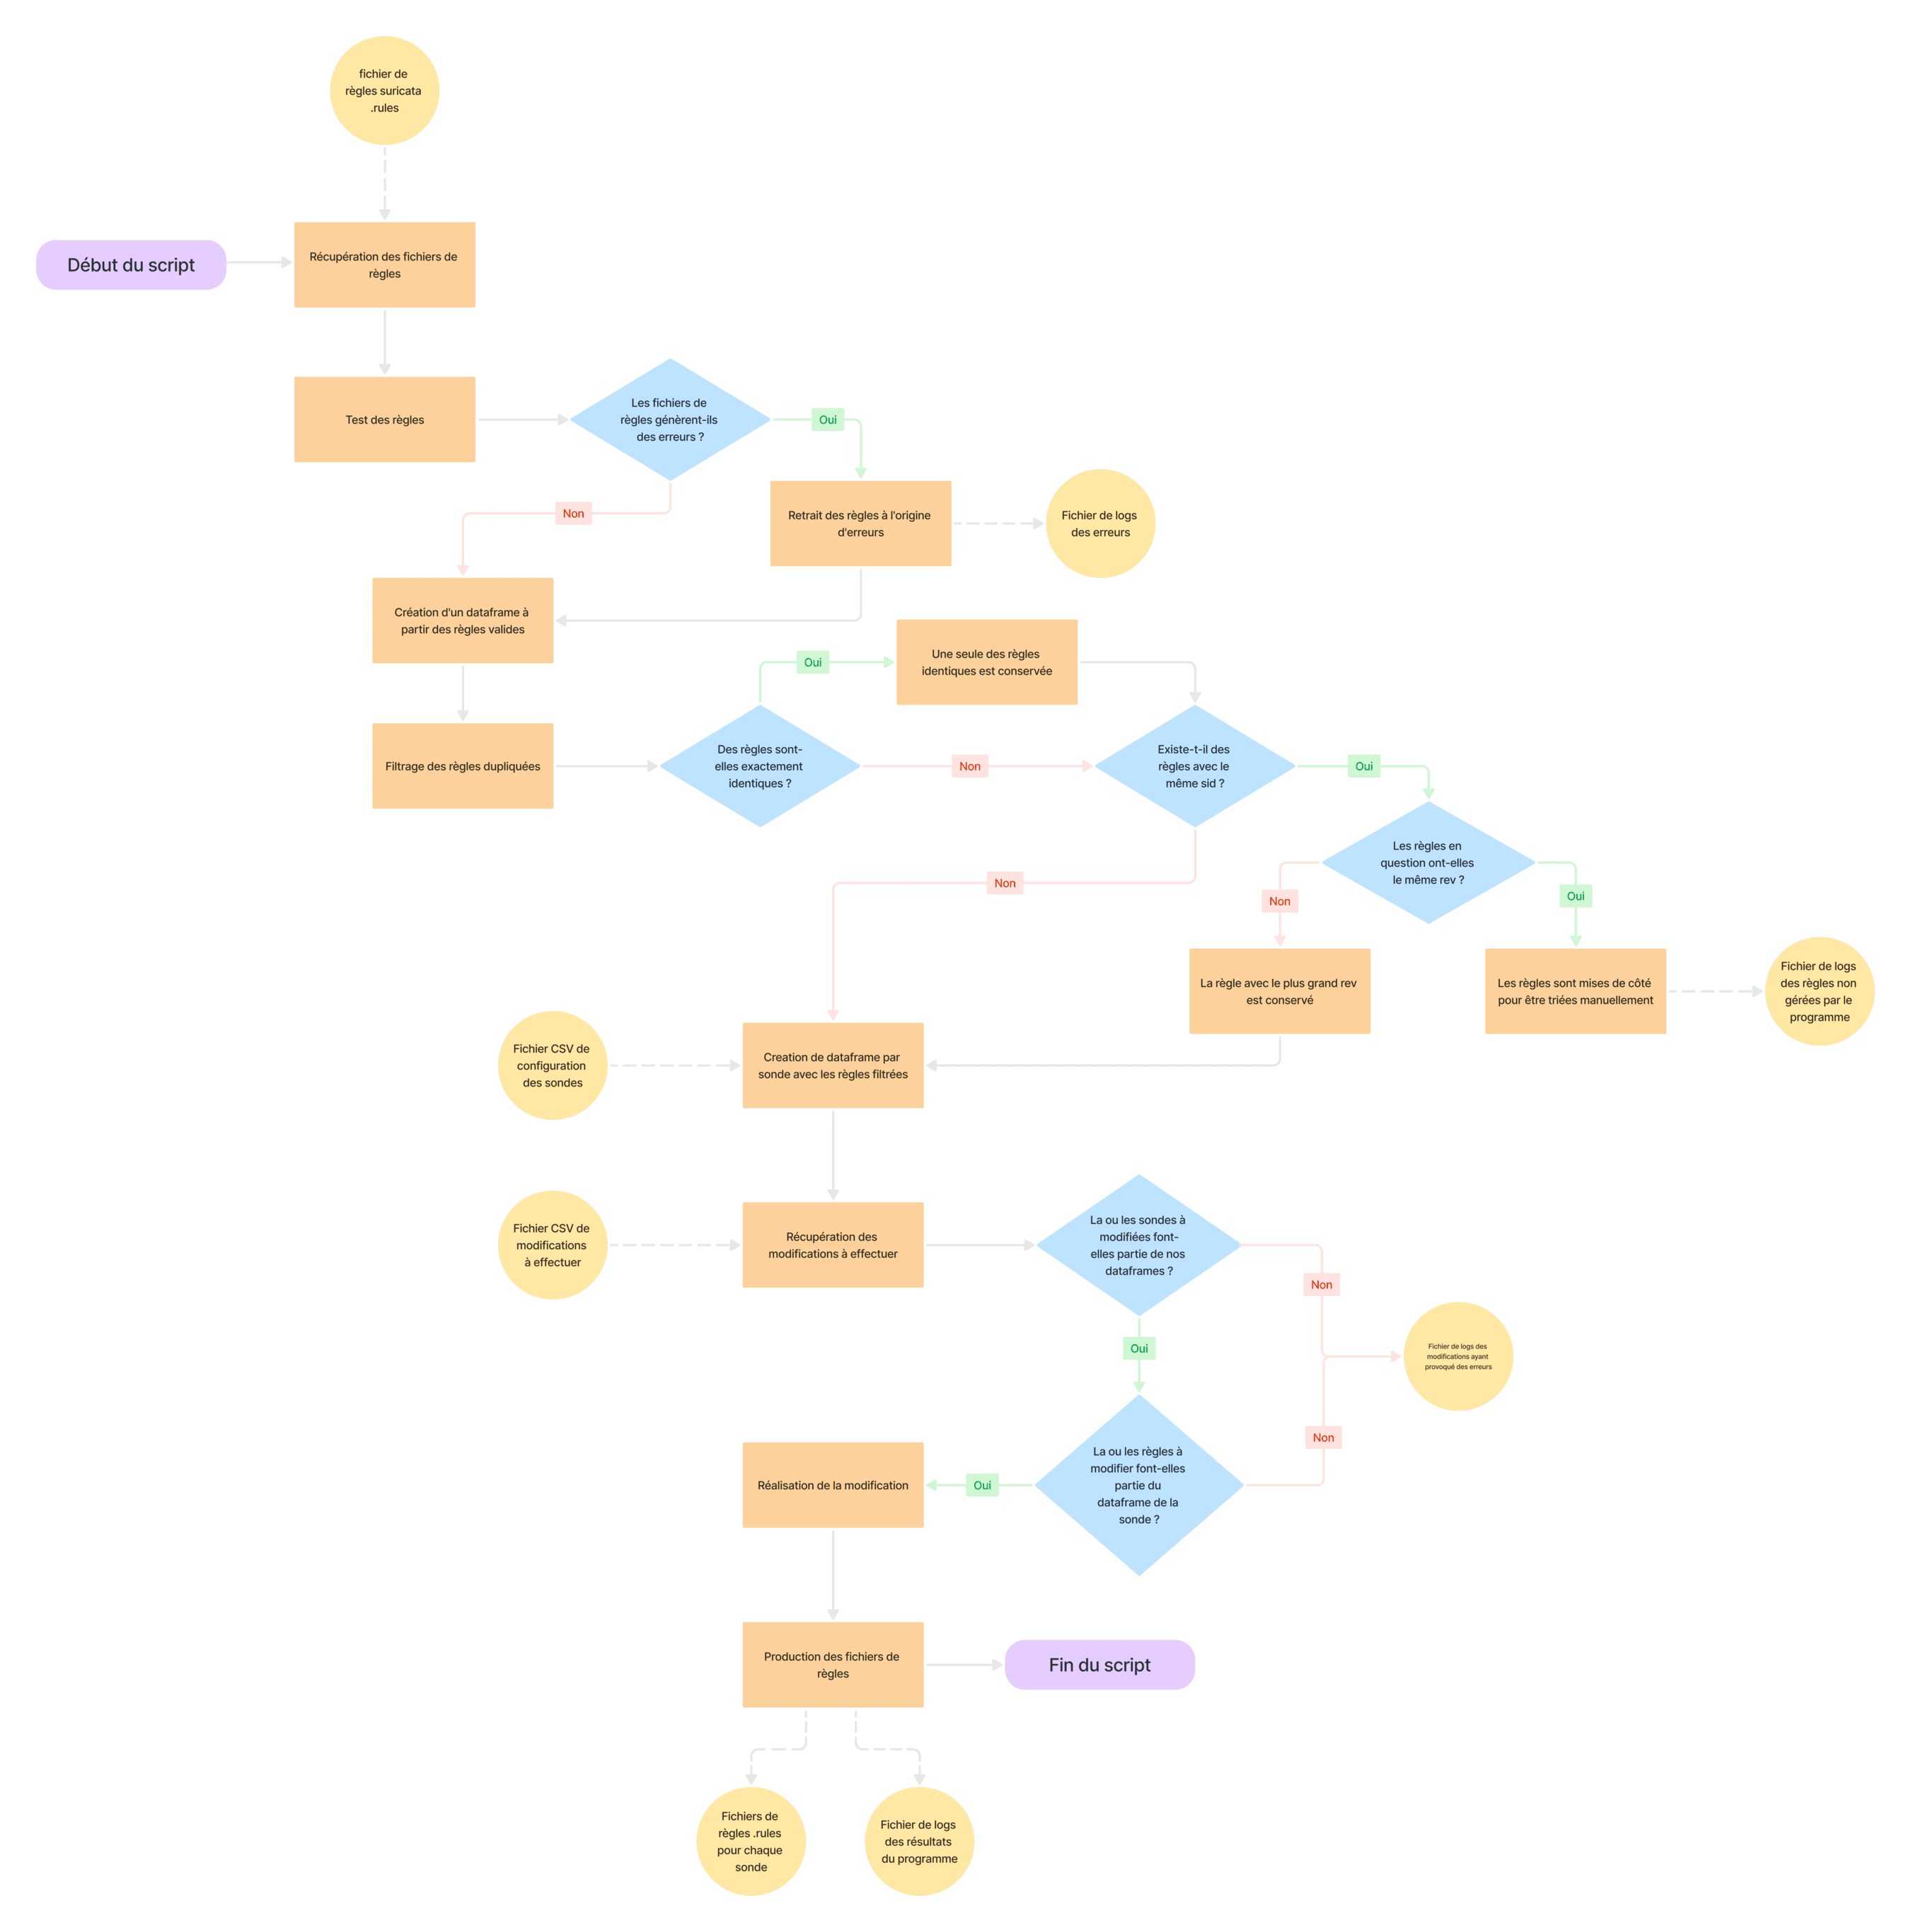
\includegraphics[width=0.97\textwidth]{assets/diagrameFlux.png}
    \caption[Diagramme de flux du programme Python développé]{Diagramme de flux du programme Python développé}\label{fig:diagrameFlux3-1.}
\end{figure}

\newpage

{\fontsize{15pt}{18pt}\selectfont
    \textbf{3.1.0 Suricata}
}

\vspace{1em}

Le programme est conçu pour récupérer les règles de Suricata uniquement. Suricata\footnote{Site officiel de Suricata : \url{https://suricata.io}} est un système de détection d'intrusion (IDS), de prévention d'intrusion (IPS) et de surveillance de la sécurité du réseau (NSM). Créé et maintenu par l'OISF\footnote{Open Information Security Foundation : \url{https://oisf.net/}}, il est utilisé au sein de l'AMSN pour ses fonctions IDS au service des objectifs de détection de l'Agence. Le choix de l'Agence s'est porté sur Suricata car il s'agit du seul outil disponible sur les sondes qualifiées par l'ANSSI.\\

Suricata fonctionne comme un \hyperref[chap2:IDSsignature]{\textbf{\textit{IDS à base de signatures}}} c'est à dire grâce à des signatures pré-configurées, des règles servant à détecter des actions malveillantes réalisées sur un réseau. Les règles Suricata se structurent ainsi en trois parties :
\vspace{0.5em}
\begin{itemize}[itemsep=0.75em]
    \item[•] Une partie \textit{action} qui stipule ce que la règle fera en cas de détection (dans ce cas, où l'Agence ne fait que de la supervision, seule l'action "alerte" est utilisée pour créer des signalements pour le SOC-MC) ;
    \item[•] Un entête dans lequel sont définis le protocole et le réseau sur lesquels la détection aura lieu ;
    \item[•] Une section \textit{option}, qui permet de définir des paramètres variables sur la règle.\\
\end{itemize}

\begin{figure}[h]%
    \center%
    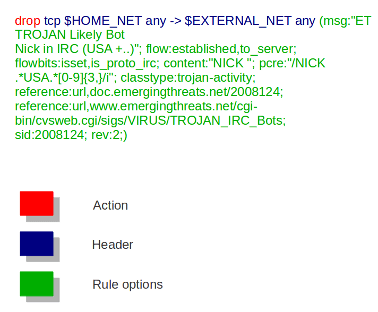
\includegraphics[width=0.5\textwidth]{assets/intro_sig.png}
    \caption[Exemple de la structure d'une règle Suricata (source: \href{https://redmine.openinfosecfoundation.org/projects/suricata/wiki/Suricata_Rules}{redmine.openinfosecfoundation.org})]{Exemple de la structure d'une règle Suricata}\label{fig:intro_sig}
\end{figure}

\newpage

Ces règles sont stockées dans des fichiers de règles \textit{.rules} (un format de fichiers texte utilisé par Suricata), lesquels sont directement fournis par des partenaires de renseignement cyber.\\

\begin{figure}[h]%
    \center%
\begin{lstlisting}[language=Python]
# This Ruleset is EmergingThreats Open optimized for suricata-7.0.3-enhanced.

alert udp $EXTERNAL_NET any -> $HOME_NET 53 (msg:"GPL DNS zone transfer UDP"; content:"|00 00 FC|"; offset:14; reference:cve,1999-0532; reference:nessus,10595; classtype:attempted-recon; sid:2101948; rev:8; metadata:created_at 2010_09_23, cve CVE_1999_0532, updated_at 2019_07_26;)

alert udp $EXTERNAL_NET any -> $HOME_NET 53 (msg:"GPL DNS named version attempt"; content:"|07|version"; offset:12; nocase; content:"|04|bind|00|"; offset:12; nocase; reference:nessus,10028; classtype:attempted-recon; sid:2101616; rev:9; metadata:created_at 2010_09_23, updated_at 2019_07_26;)

alert udp $EXTERNAL_NET any -> $HOME_NET 53 (msg:"GPL DNS named iquery attempt"; content:"|09 80 00 00 00 01 00 00 00 00|"; depth:16; offset:2; reference:bugtraq,134; reference:cve,1999-0009; reference:url,www.rfc-editor.org/rfc/rfc1035.txt; classtype:attempted-recon; sid:2100252; rev:9; metadata:created_at 2010_09_23, cve CVE_1999_0009, updated_at 2019_07_26;)

alert udp $EXTERNAL_NET any -> $HOME_NET 53 (msg:"GPL DNS named authors attempt"; content:"|07|authors"; offset:12; nocase; content:"|04|bind|00|"; offset:12; nocase; reference:nessus,10728; classtype:attempted-recon; sid:2100256; rev:8; metadata:created_at 2010_09_23, updated_at 2019_07_26;)

...
\end{lstlisting}
    \caption[Exemple de fichier de règles (source: \href{https://rules.emergingthreats.net/open/suricata-7.0.3/rules/emerging-dns.rules}{emerging-dns.rules})]{Exemple de fichier de règles}\label{fig:ExampleRulesFile.png}
\end{figure}


\newpage

\subsection{Récupération des règles}

\vspace{1em}

Ces fichiers de règles précédemment cités, sont mis à disposition du programme pour permettre leur centralisation. L'enjeu de rassembler les règles en un seul endroit est de s'assurer que l'outil soit capable de modifier les règles et de les envoyer aux sondes consécutivement.\\

\begin{figure}[h]%
    \center%
    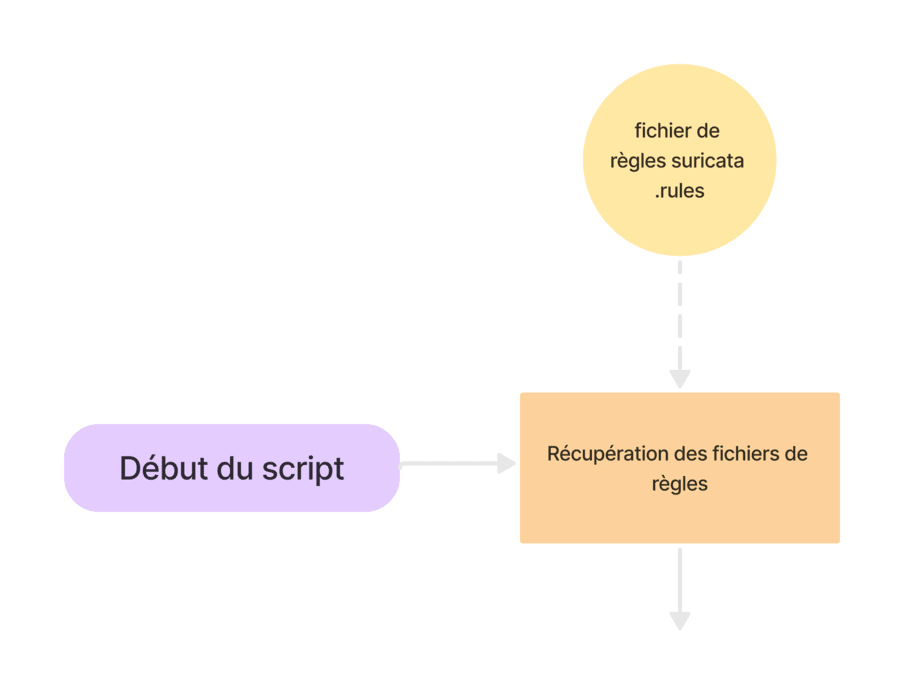
\includegraphics[width=0.7\textwidth]{assets/diagrameFlux3-1.png}
    \caption[Diagramme de flux de la section responsable de la récupération des règles]{Diagramme de flux de la section responsable de la récupération des règles}\label{fig:diagrameFlux3-1}
\end{figure}

\vspace{1em}

Le script a été conçu pour récupérer en entrée un dossier positionné à la racine du programme avec les fichiers de règles qui seront lus par le programme.\\

\begin{figure}[h]%
    \center%
\begin{lstlisting}[language=Python]
# Parcours chaque fichier dans le repertoire fourni
for filepath in os.listdir("rules"):
    suricata_alerts = extract_suricata_alerts(filepath)
\end{lstlisting}
    {\small
    \textit{Traite chaque fichier de règles individuellement depuis le dossier "rules"}
    }
    \caption[Récupération des règles]{Récupération des règles}
\end{figure}

Chaque fichier présent dans le dossier va être testé puis ensuite les règles seront récupérées et rassemblées.

\newpage

\subsection{Contrôle des règles en entrée}

\vspace{1em}

Avant la récupération des règles, le programme doit être capable de tester les règles récupérées car selon les retours des membres du CERT-MC, il arrivait que des erreurs (faute de frappe, mauvaise valeur inscrite...) soient contenues dans les règles de détection des fichiers récupérés ou que lesdites règles soient destinées à une version de Suricata qui n'est pas compatible avec celles des sondes. Ce qui pouvait provoquer le blocage d'une sonde si les règles en question arrivaient en bout de chaîne.\\

\vspace{0.5em}

Pour cette raison il était attendu de mon programme qu'il soit capable de contrôler la validité des règles avec les sondes pour prévenir, en cas de panne, le risque de perte en capacité de détection.\\

\begin{figure}[h]%
    \center%
    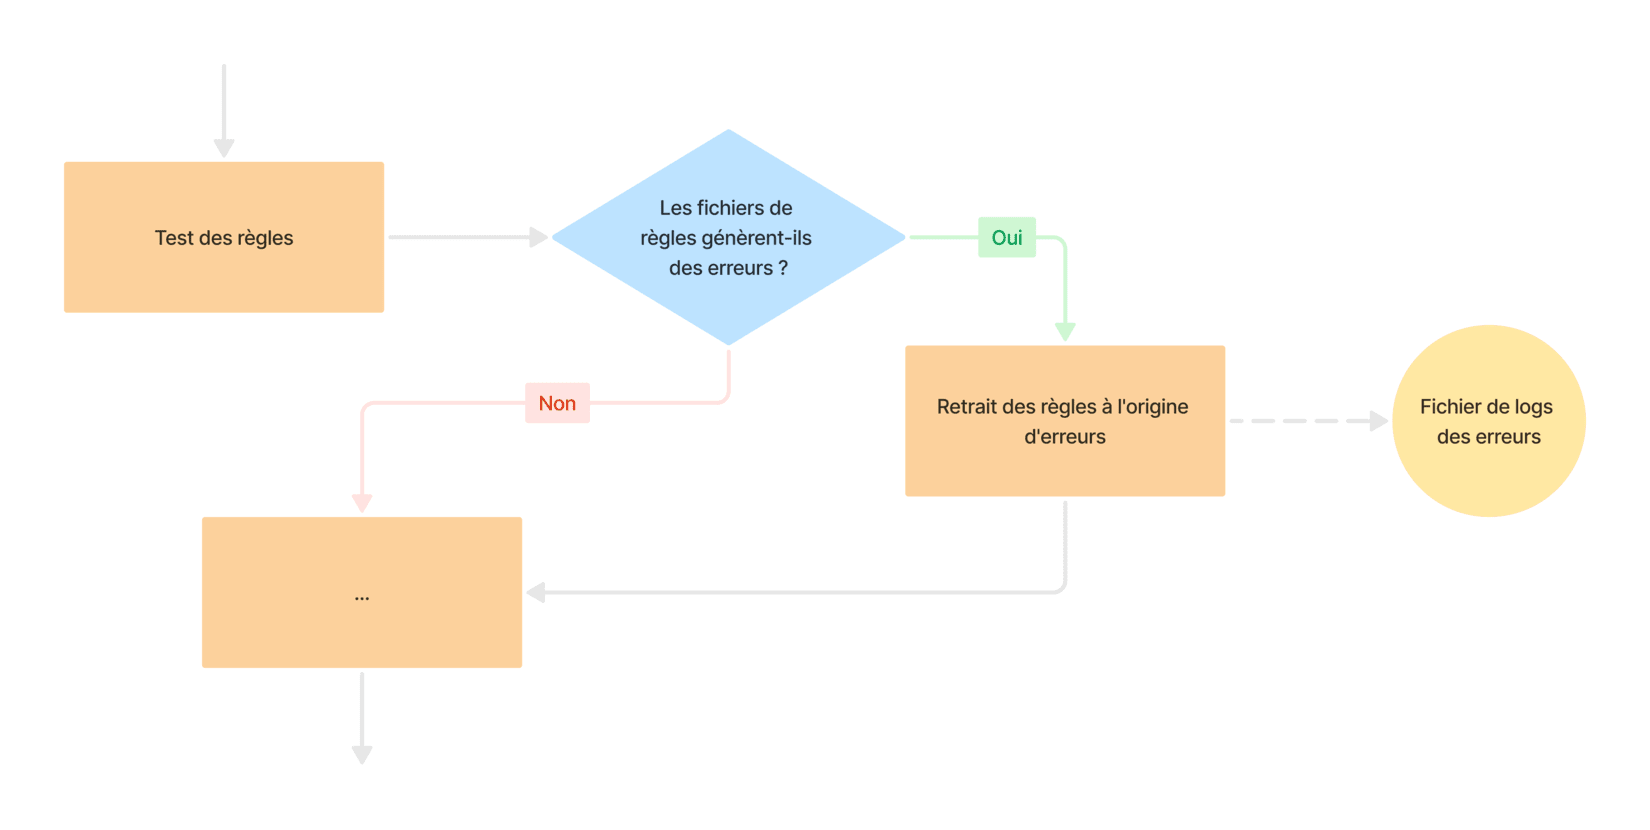
\includegraphics[width=1\textwidth]{assets/diagrameFlux3-2.png}
    \caption[Diagramme de flux de la section responsable du contrôle des règles]{Diagramme de flux de la section responsable du contrôle des règles}\label{fig:diagrameFlux3-2}
\end{figure}

\vspace{1em}

Le programme va ainsi tester individuellement chaque fichier récupéré. Pour cela Suricata dispose d'un mode test qui permet de compiler un fichier de règles. A cette fin, une version de Suricata comparable à celle présentée sur les sondes a été installée localement sur mon poste de travail. 

\newpage

\begin{figure}[h]%
    \center%
\begin{lstlisting}[language=Python]
testresult = subprocess.run(['suricata', '-T', '-c', 'configTestSuricata.yaml','-l', '/tmp/', '-S', filepath], capture_output=True, text=True)
\end{lstlisting}
    {\small
    \textit{Teste le fichier présent dans la variable "filepath" en utilisant la version locale de Suricata et le fichier de configuration 'configTestSuricata.yaml’ \hyperref[chap:annexe1]{[A.1]}}
    }
    \caption[Test des fichiers de règles]{Test des fichiers de règles}\label{fig:TestFileRule}
\end{figure}

\vspace{1em}

Pour chaque fichier testé, la version locale de Suricata génère des journaux d'erreurs qui désignent chaque règle ayant provoqué des erreurs avec une description de celle-ci \hyperref[chap:annexe2]{[A.2]}. A partir de ces journaux des résultats des tests, j'identifie les potentielles règles défectueuses.\\

\begin{figure}[h]%
    \center%
    \begin{lstlisting}[language=Python]
# Si le fichier produit une erreur
if (testresult.returncode == 1):
    # 'stderr' = toute les erreurs qui ont encourue
    for line in testresult.stderr.split('\n'):
        if line.startswith('E: detect: error parsing signature'):
            # Extraction de la ligne des messages d'erreur
            linenumber = line.split(' ')[-1]
            line_to_remove.append(int(linenumber))
            # Recuperation des erreurs pour creation csv
            csvError["collumnRules"].append(line)
        else:
            csvError["collumnError"].append(line)
\end{lstlisting}
    {\small
    \textit{Parcours de chaque ligne des journaux d'erreurs pour dénombrer les lignes non fonctionnelles. "Linenumber" est la variable qui stocke les numéros des lignes des règles qui provoquent des erreurs.}
    }
    \caption[Identification des règles ayant provoqué des erreurs]{Identification des règles ayant provoqué des erreurs}\label{fig:IdentRulesError}
\end{figure}

\vspace{1em}

Celles-ci seront mises de côté pour la prochaine mise à jour des sondes pour n'utiliser que les valides pour le reste du programme.\\

\begin{figure}[h]%
    \center%
    \begin{lstlisting}[language=Python]
# Boucle dans les fichiers de regles
with open(filepath, 'r') as file:
    for i, line in enumerate(file, start=1):
        # On ne garde que les lignes qui ne font pas partie des erreurs
        if i not in line_to_remove and line.startswith("alert "):
            suricata_alerts.append({'rules': line, 'source': sourceName})

return suricata_alerts
\end{lstlisting}
    {\small
    \textit{Parcours à nouveau du fichier de règles testé, en supprimant toutes les lignes qui ont été détectées comme étant à l'origine d'erreurs. "suricata\_alerts", les règles finales récupérées.}
    }
    \caption[Récupération des règles en excluant les erreurs]{Récupération des règles en excluant les erreurs}\label{fig:GetRules}
\end{figure}

\newpage

Afin de pouvoir tenir compte des règles qui commettent des erreurs au fil du temps, celles-ci sont stockées dans des fichiers CSV (Figure 3.12) avec leur code d'erreur. Cela permet d'établir des statistiques sur le taux de règles valides envoyées par les partenaires de renseignement sur la menace.\\

\subsubsection{\textit{Note}}
Le format CSV a été choisi pour stocker les informations relatives aux fichiers de configuration et aux résultats du programme. Ce format est utilisé parce qu'il est compatible avec Excel et Splunk, deux logiciels largement utilisés au sein de l'Agence.

\newpage

\subsection{Filtrage des règles}

\vspace{1em}

Une fois que les règles non valides ont été supprimées de l'ensemble traité, un autre problème se pose. Par la multitude de fournisseurs de règles, il existe le risque que la même règle (ayant probablement été établie à partir du même IOC) soit partagée par plusieurs partenaires différents. C'est pourquoi, pour éviter la surcharge inutile des sondes, il m'a été demandé de permettre à l'outil développé de filtrer les règles dupliquées.\\

\begin{figure}[h]%
    \center%
    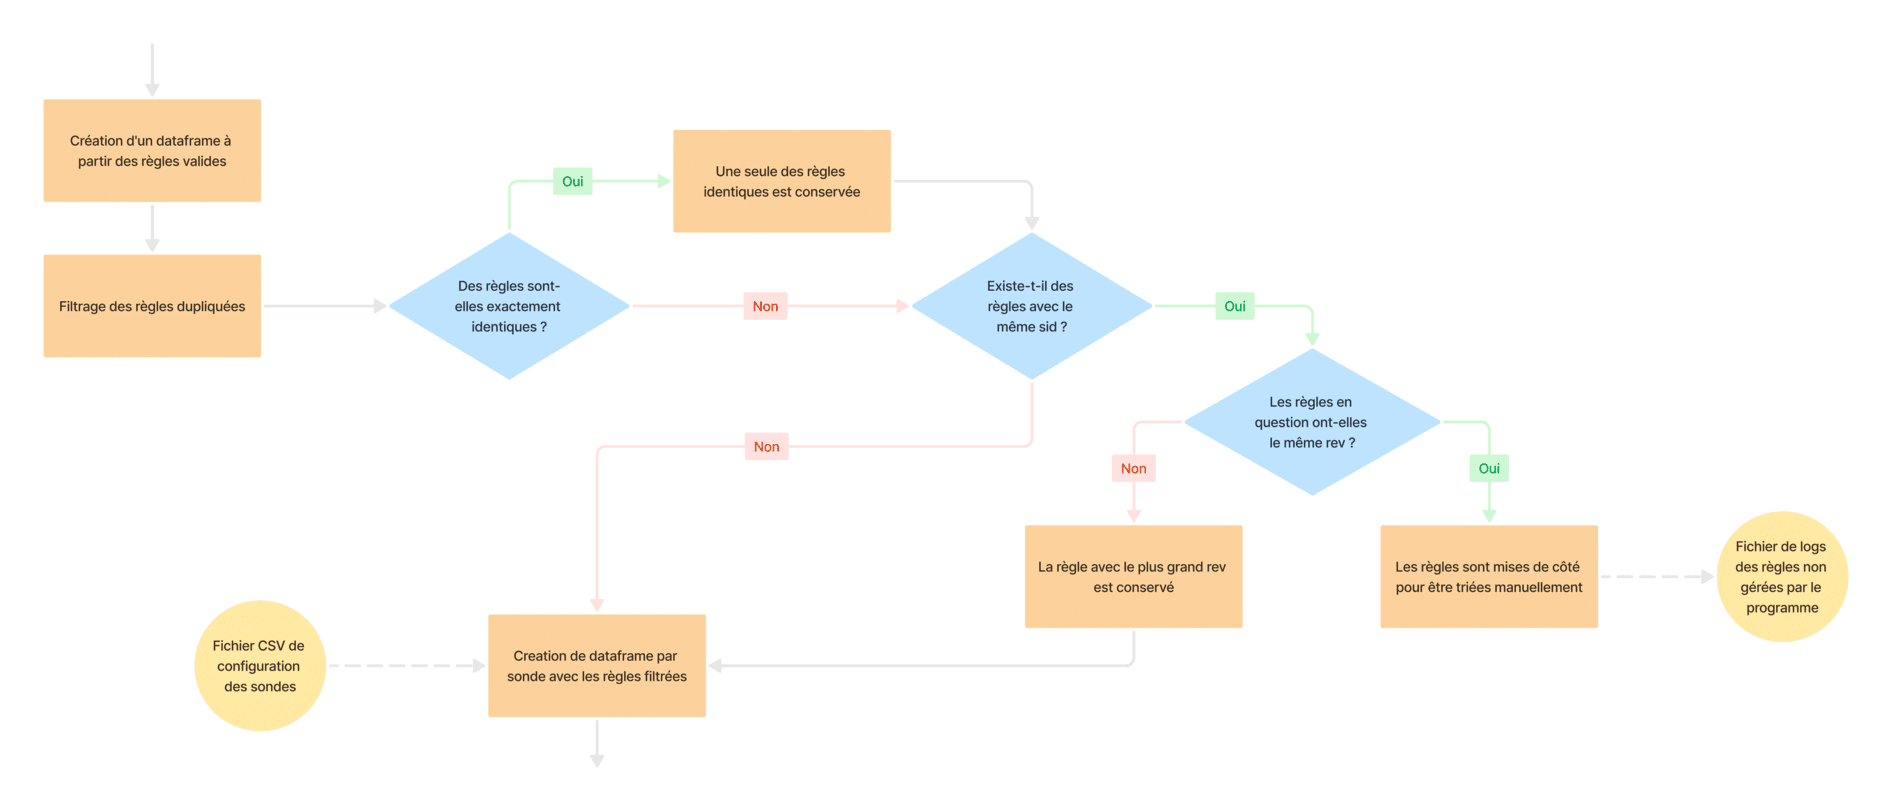
\includegraphics[width=1\textwidth]{assets/diagrameFlux3-3.png}
    \caption[Diagramme de flux de la section responsable du filtrage des règles]{Diagramme de flux de la section responsable du filtrage des règles}\label{fig:diagrameFlux3-3}
\end{figure}

\vspace{1em}

Pour mener à bien cette tâche (ainsi que d'autres manipulations que le programme devra appliquer à ces données par la suite), j'ai eu besoin d'utiliser une bibliothèque logicielle de data-science : \textit{pandas}\footnote{Pandas est une bibliothèque open-source flexible d'analyse et de manipulation de données pour Python : \url{https://pandas.pydata.org/}}. Elle permet de créer des ensembles de structures de données bidimensionnelles, \textit{dataframes}, qui permettent au programme de rassembler toutes les règles dans une seule variable et d'appliquer des modifications à l'ensemble en quelques lignes de code seulement.\\

\newpage

\begin{figure}[h]%
    \center%
\begin{lstlisting}[language=Python]
#Import de la librairie
import pandas as pd

Dataframe_alerts = pd.DataFrame(suricata_alerts)
\end{lstlisting}
    {\small
    \textit{Importation de la bibliothèque Pandas et création d'un \textit{dataframe} à partir de "suricata\_alerts", une liste composée de toutes les règles récupérées jusqu'à présent.}
    }
    \caption[Création de dataframe \textit{pandas}]{Création de dataframe \textit{pandas}}\label{fig:CreateDataf}
\end{figure}

\subsubsection{\textit{Note}}
J'avais initialement essayé de réaliser ce programme en utilisant uniquement les outils fournis par défaut par Python, mais la taille colossale des données à traiter (plusieurs dizaines de milliers de règles) a rendu cette option inefficace et a provoqué un ralentissement excessif de l'exécution du programme. Cela m'a contraint à recourir à des outils de traitement de données. Le choix s'est porté sur Pandas car il s'agit d'une bibliothèque reconnue pour sa performance et qui est régulièrement maintenue.\\

\vspace{0.5em}

Grâce à cette bibliothèque, le processus de filtrage s'est déroulé en deux étapes. Tout d'abord, les règles qui sont strictement identiques à d'autres sont supprimées.\\

\begin{figure}[h]%
    \center%
\begin{lstlisting}[language=Python]
# Trouve toutes les regles strictement en double pour n'en garder qu'une
duplicates = allrules[allrules.duplicated('rules', keep=False)]
if duplicates.empty == False:
    grouped = duplicates.groupby('rules')['source'].agg(', '.join).reset_index()
    allrules = pd.concat([allrules[~allrules['rules'].isin(duplicates['rules'])], grouped], ignore_index=True)
\end{lstlisting}
    \caption[Suppression des règles dupliquées]{Suppression des règles dupliquées}\label{fig:DeleteRules}
\end{figure}

\vspace{1em}

Puis elles sont triées en fonction du \textit{sid} et de la \textit{rev} des règles.
Cette seconde étape est due au fonctionnement de Suricata qui exige que la section \textit{options} des règles comporte une variable \textit{sid} (pour signature ID) unique à chaque règle, qui est utilisée pour les identifier. Comme les partenaires de l'Agence respectent les conventions d'écriture des règles et en particulier les plages d'allocation de \textit{sid}\footnote{\url{https://sidallocation.org/}}, différentes règles ayant le même \textit{sid} sont nécessairement basées sur le même IOC et le programme n'a plus qu'à décider lequel conserver.\\

\newpage

Pour départager deux règles ayant le même \textit{sid}, j'utilise une autre variable présente dans les options des règles Suricata \textit{rev} (pour revision) qui sert à spécifier un numéro de version d'une règle. La règle ayant la valeur numérique de sa variable \textit{rev} la plus élevée est la règle qui à été mise à jour en dernier et sera donc privilégiée.\\

\vspace{0.5em}

\begin{figure}[h]%
    \center%
\begin{lstlisting}[language=Python]
# On ceer une collone sid dans le dataframe a partir des sid des regles
allrules['sid'] = allrules['rules'].str.extract(r'sid:(.*?);')

# On trouve toutes les sid n'etant pas unique dans le dataframe
conflictedrules = allrules[allrules.duplicated('sid', keep=False)]

# Creation d'une nouvelle collone rev pour priorisation par rev
conflictedrules['rev'] = conflictedrules['rules'].str.extract(r'rev:(.*?);').astype(int)
# Groupe par 'sid'
grouped = conflictedrules.groupby('sid')
# Groupe par 'rev'
max_rev_per_group = grouped['rev'].max()

# Garde pour chaque sid la regle ayant la plus haute rev. si des regle on la meme sid et rev elles seront non resolu
conflictedrules = conflictedrules[conflictedrules.apply(lambda x: x['rev'] == max_rev_per_group[x['sid']], axis=1)]
\end{lstlisting}
    \caption[Gestions des règles en collision de sid]{Gestions des règles en collisions de sid}\label{fig:HandlingCollisions}
\end{figure}

\vspace{0.5em}

Une fois le tri terminé, de nouveaux \textit{dataframmes} sont créés pour correspondre au nombre de sondes qui recevront des fichiers de règles en sortie du programme. Ces différents \textit{dataframmes} sont utilisés pour appliquer des modifications aux règles en fonction des sondes cibles.

\vspace{1em}

\begin{figure}[h]%
    \center%
\begin{lstlisting}[language=Python]
# creer un dataframes de regles pour chaque sonde
rulesByProbes = {}
for name in SondesNames:
   rulesByProbes[name[0]] = cleanedrules[:]
\end{lstlisting}
{\small
    \textit{Crée un dictionnaire d'images de données pour chaque sonde finale.}
    }
    \caption[Création de dataframe pour chaque sonde]{Création de dataframe pour chaque sonde}\label{fig:CreateDatafBySonde}
\end{figure}

\newpage

\subsection{Modification des règles}
\label{chap3:section1rulesmodif}

\vspace{1em}

Les membres du SOC-MC m'avaient fait part de leur besoin d'acquérir la capacité de modifier facilement les ensembles de règles. Les analystes du SOC-MC observent lors de leur travail quotidien l'efficacité des règles mises en place sur les sondes. Leurs observations et enquêtes ont mis en évidence des règles inutiles ou trop "bruyantes" que mon programme devait être capable de modifier.

\begin{figure}[h]%
    \center%
    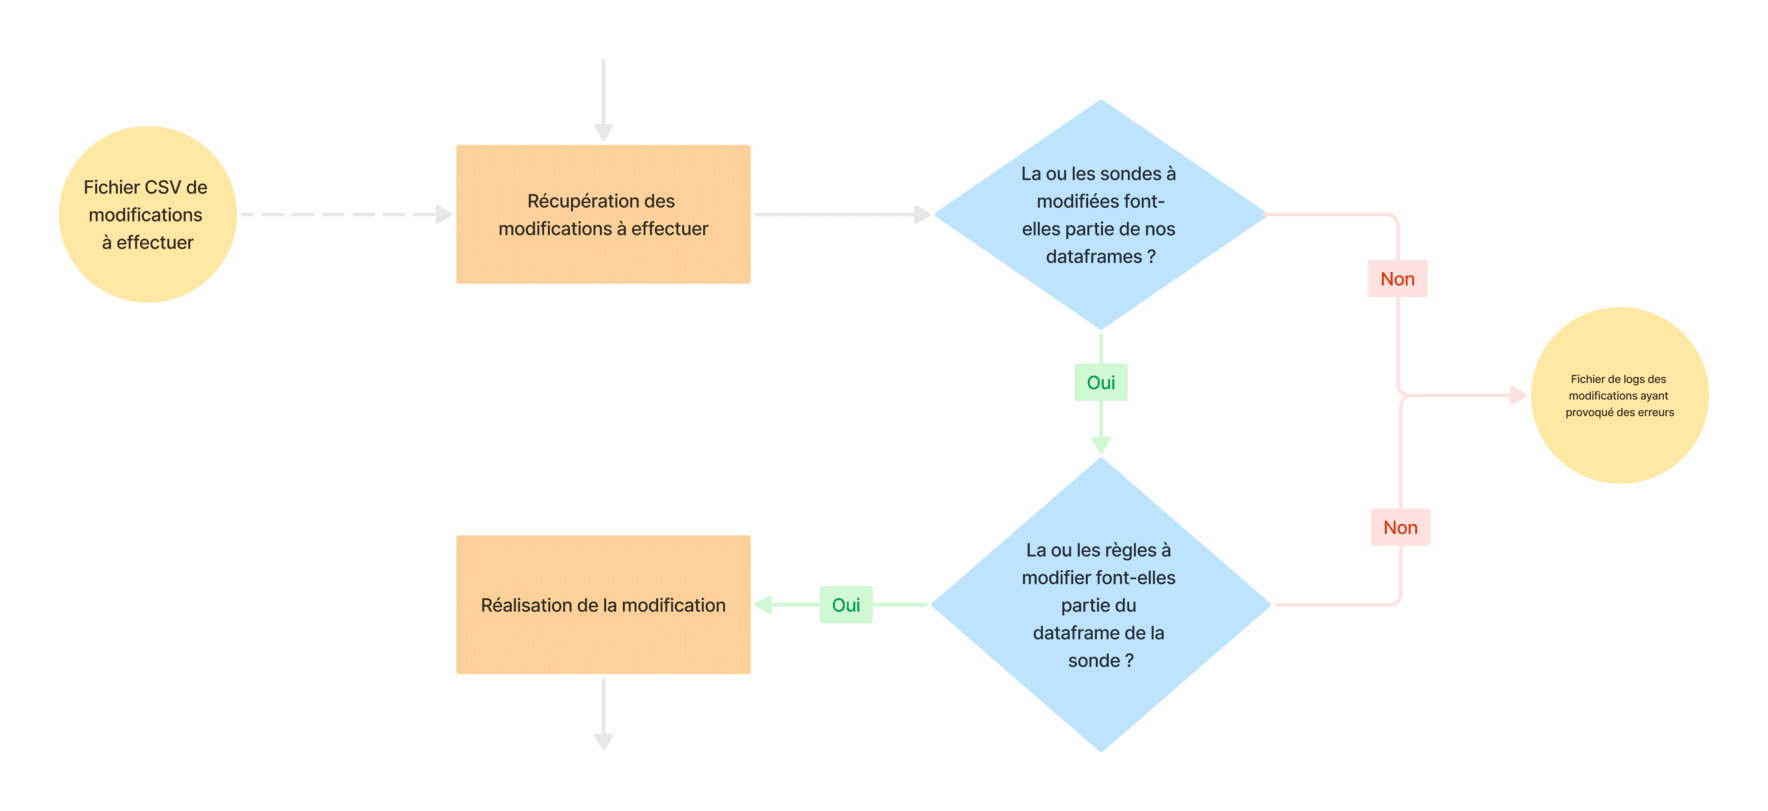
\includegraphics[width=1\textwidth]{assets/diagrameFlux3-4.png}
    \caption[Diagramme de flux de la section responsable de l'application des modifications]{Diagramme de flux de la section responsable de l'application des modifications}\label{fig:diagrameFlux3-4}
\end{figure}

\vspace{1em}

Les modifications à effectuer sont fournies au programme sous la forme d'un fichier CSV stipulant les règles à rectifier en fonction de leur \textit{sid} ainsi que l'amendement à apporter et pour quelle sonde l'appliquer. Ce fichier est complété soit par les analystes SOC, soit par d'autres membres du CERT-MC sur la base de leurs constatations quant à l'efficacité des règles sur les sondes.\\

\vspace{1em}

\begin{figure}[h]%
    \center%
    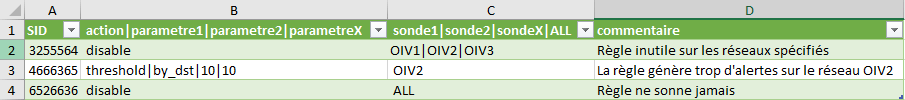
\includegraphics[width=1\textwidth]{assets/CaptureCSV.png}
    \caption[Exemple de fichier CSV de configuration des règles à modifier]{Exemple de fichier CSV de configuration des règles à modifier}\label{fig:CaptureCSV}
\end{figure}

\newpage

Le programme récupère le contenu du fichier et désactive les règles ou applique des seuils pour réduire le nombre d'alertes qu'elles génèrent (des "threshold" dans la terminologie de Suricata).\\

\begin{figure}[h]%
    \center%
\begin{lstlisting}[language=Python]
# On applique la modification
if (changeToApply == "disable"):
    # Pour 'disable' on enleve la regle de la liste
    rulesByProbes[sonde[0]] = rulesByProbes[sonde[0]][rulesByProbes[sonde[0]]["sid"] != targetSid]
elif len(changeToApply) > 3:
    # Hors 'disable' il s'agit d'un changement de threshold
    # On cree la nouvelle option
    changeToApply = "threshold: type " + changeToApply[0] + ", track " + changeToApply[1] + ", seconds " + changeToApply[3] + ", count " + changeToApply[2] + ";"
    # rulesToChange = la regle qui va etre modifiee
    rulesToChange = rulesByProbes[sonde[0]].loc[rulesByProbes[sonde[0]]["sid"] == targetSid, 'rules']
    # On modifie la section msg de la regle pour notifier qu'elle a ete modifiee
    rulesToChange = rulesToChange.str.replace('msg:"', 'msg:"AMSN_RULE ')
    # Si l'option threshold existe deja dans rulesToChange on la remplace par la nouvelle
    if (re.search('threshold:', rulesToChange.tolist()[0])):
        rulesToChange = rulesToChange.str.replace(r'threshold:(.*?);', changeToApply, regex=True)
    # S'il n'y a pas d'option threshold dans la regle modifiee on place la nouvelle option a la fin 
    else:
        rulesToChange = rulesToChange.values[0].rsplit(')', 1)[0] + changeToApply + ')\n'
    # on reincopore la regle modifiee dans le dataframe de la sonde selectionnee
    rulesByProbes[sonde[0]].loc[rulesByProbes[sonde[0]]["sid"] == targetSid, 'rules'] = rulesToChange
\end{lstlisting}
{\small
    \textit{Modifie les règles en écrivant à l'intérieur les nouvelles valeurs dans le cas de changement de 'threshold' et retire la règle du dataframe dans le cas d'un changement 'disable'.}
    }
\caption[Modifications des règles]{Modifications des règles}\label{fig:ModifRules}
\end{figure}

\vspace{1em}

Ces seuils sont une option activée par Suricata, permettant de limiter le nombre d'alertes par minute générées par une règle. Les modifications ne sont apportées qu'aux \textit{dataframes} destinés aux sondes spécifiées dans le fichier CSV, permettant une différenciation par OIV.

\newpage

\subsection{Traitement des résultats}

\vspace{1em}

Afin de répondre aux exigences de l'Agence, le programme doit utiliser les opérations précédentes pour générer un fichier de règles, pour chaque sonde destinataire, qui puisse être exporté facilement. En outre, pour permettre à l'Agence de suivre les résultats du programme dans le temps, j'ai dû mettre en place un système de journalisation dans le code.

\begin{figure}[h]%
    \center%
    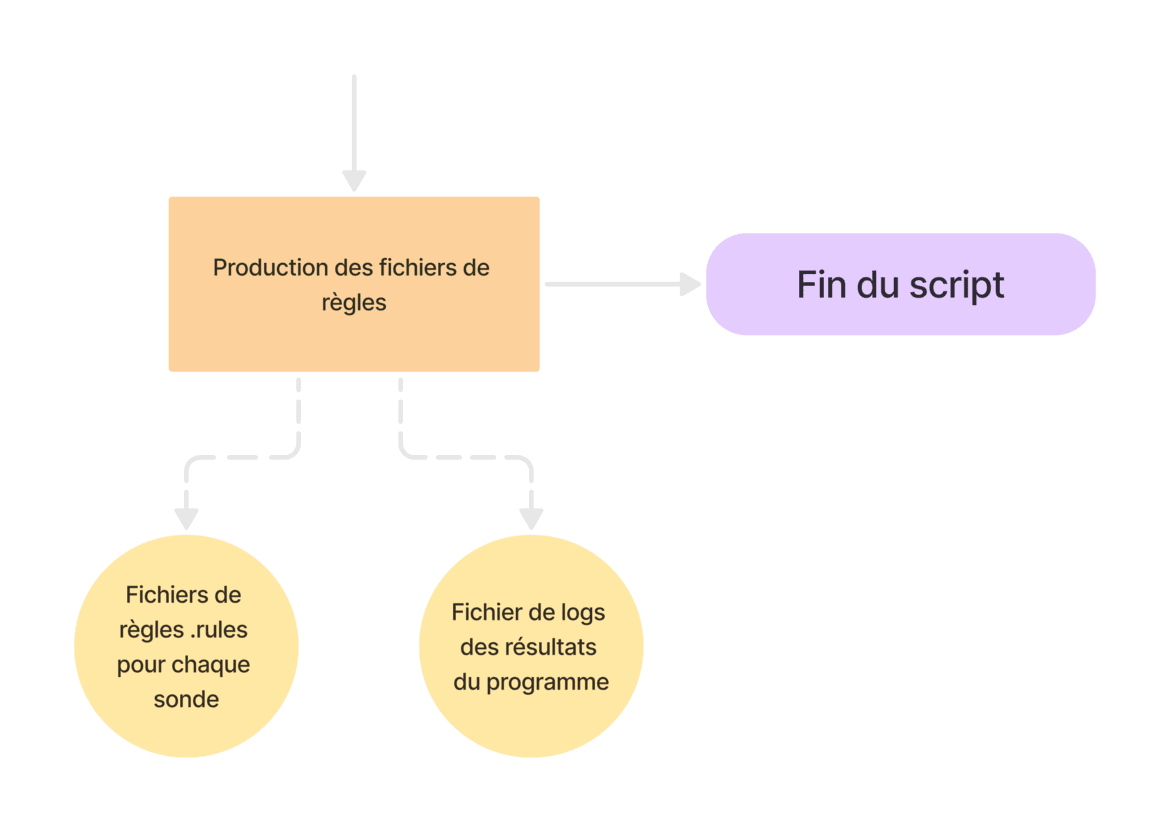
\includegraphics[width=0.8\textwidth]{assets/diagrameFlux3-5.png}
    \caption[Diagramme de flux de la fin du programme]{Diagramme de flux de la fin du programme}\label{fig:diagrameFlux3-5}
\end{figure}

\vspace{1em}

À partir des \textit{dataframes} mentionnés précédemment, un fichier de règles a été généré pour chaque sonde et est stocké dans un dossier distinct afin de pouvoir être exporté vers le système de gestion des sondes.\\

\newpage

\begin{figure}[h]%
    \center%
\begin{lstlisting}[language=Python]
### AMSN generated rules files ###

alert udp any any -> $HOME_NET 139 (msg:"ET NETBIOS Microsoft Windows NETAPI Stack Overflow Inbound - MS08-067 (1)"; content:"|0B|"; offset:2; depth:1; content:"|C8 4F 32 4B 70 16 D3 01 12 78 5A 47 BF 6E E1 88|"; reference:url,www.microsoft.com/technet/security/Bulletin/MS08-067.mspx; reference:cve,2008-4250; reference:url,www.kb.cert.org/vuls/id/827267; classtype:attempted-admin; sid:2008690; rev:5;  metadata: amsn_source gcenter_netbios, created_at 2010_07_30, cve CVE_2008_4250, updated_at 2017_11_22;)

alert tcp $EXTERNAL_NET any -> $HOME_NET 139 (msg:"ET NETBIOS Microsoft SMB NetLogon UUID detected Big Endian SET"; flow:to_server,established; content:"|ff|SMB"; content:"|05 00 0b|"; distance:0; byte_test:1,!&,0x10,1,relative; content:"|12345678 1234 abcd ef00 01234567cffb|"; distance:29; flowbits:set,smb.netlogon.uuid.detected; flowbits:noalert; reference:cve,2010-2742; reference:url,www.microsoft.com/technet/security/bulletin/MS10-101.mspx; classtype:attempted-user; sid:2800985; rev:2;  metadata: amsn_source gcenter_netbios, created_at 2010_12_15, cve CVE_2010_2742, updated_at 2017_11_22;)

...
\end{lstlisting}
    \caption[Exemple de fichier de règles généré]{Exemple de fichier de règles généré}\label{fig:captureOIVrules}
\end{figure}

\vspace{1em}

Pour pouvoir répondre au besoin d'information sur les résultats du programme, j'ai mis en place une journalisation via la génération de CSV tout au long de l'exécution du programme :\\

\vspace{1em}

\begin{itemize}[itemsep=2em]
    \item[•] Lorsque les règles récupérées sont testées, un fichier CSV est créé pour enregistrer les règles qui ont été détectées comme étant à l'origine d'erreurs et leurs sources.

\vspace{1em}

    \begin{figure}[h]%
        \center%
        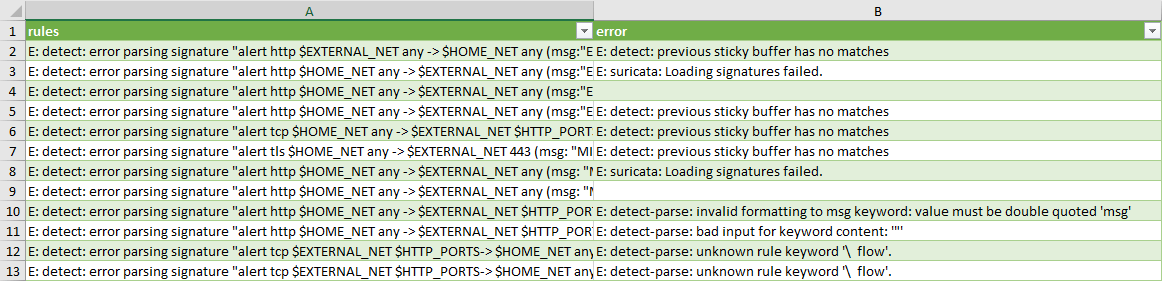
\includegraphics[width=0.9\textwidth]{assets/SuricataError.png}
        \caption[Exemple de fichier CSV d'erreurs dans les fichiers testés]{Exemple de fichier CSV d'erreurs dans les fichiers testés}\label{fig:SuricataError}
    \end{figure}

\newpage

    \item[•] Lorsque les règles en double sont filtrées, un fichier CSV est créé pour les règles potentielles qui ne peuvent pas être gérées automatiquement en vue d'un tri manuel.

\vspace{1em}

    \begin{figure}[h]%
        \center%
        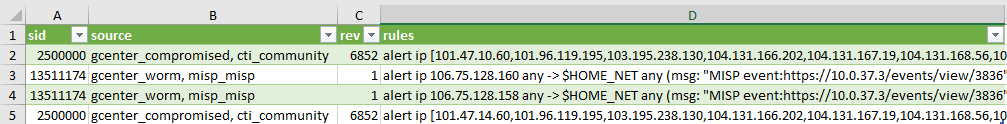
\includegraphics[width=1\textwidth]{assets/RuleColision.png}
        \caption[Exemple de fichier CSV de règles dupliquées non géré]{Exemple de fichier CSV de règles dupliquées non gérées}\label{fig:RuleColision}
    \end{figure}

    \item[•] Lorsque les modifications demandées par le personnel du CERT-MC sont appliquées, les modifications qui n'ont pas pu être effectuées (en raison d'une erreur dans les fichiers de configuration) sont sauvegardées dans un fichier CSV.\\

\vspace{1em}

    \begin{figure}[h]%
        \center%
        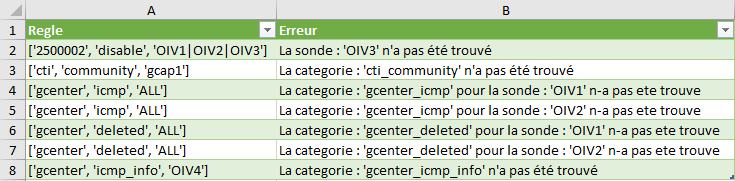
\includegraphics[width=0.8\textwidth]{assets/ErrorModif.png}
        \caption[Exemple de fichier CSV d'erreur de modification de règle]{Exemple de fichier CSV d'erreur de modification de règle}\label{fig:ErrorModif}
    \end{figure}

\vspace{1em}

    \item[•] Lorsque le programme est terminé, un fichier de statistiques générales est généré.\\

\newpage

    \begin{figure}[h]%
        \center%
        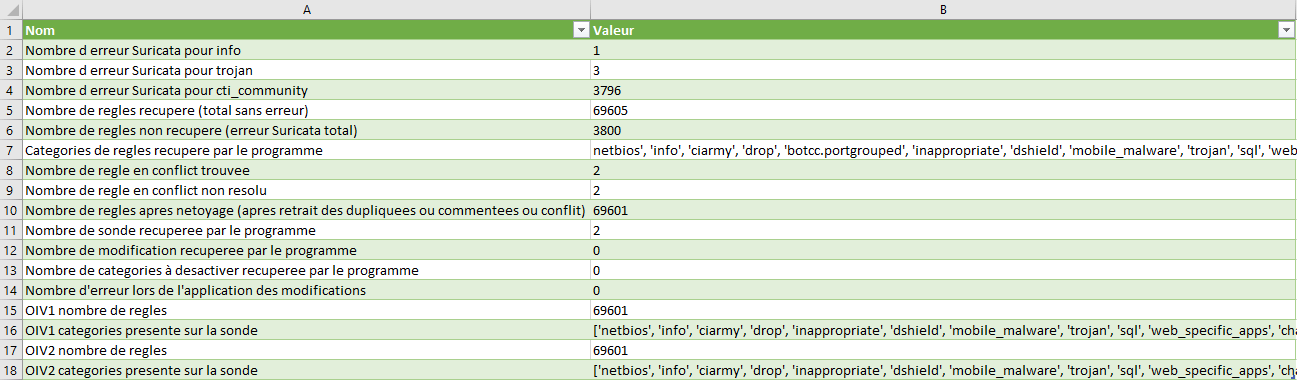
\includegraphics[width=1\textwidth]{assets/stat.png}
        \caption[Exemple de fichier CSV de statistiques du programme]{Exemple de fichier CSV de statistiques du programme}\label{fig:Stat}
    \end{figure}

\end{itemize}

\vspace{1em}

Ces fichiers sont générés à chaque mise à jour des sondes et sont stockés séparément par date. Les fichiers ainsi créés permettent de comparer les résultats des différentes mises à jour des sondes et de suivre dans le temps quelles règles étaient actives sur chaque sonde à un moment donné.\\

L'importance de développer cette capacité est de permettre au programme de répondre à certaines exigences du référentiel \textit{PDIS}\footnote{\textit{"Le prestataire doit élaborer et tenir à jour pour chaque commanditaire la liste de l’ensemble des règles de détection mises en œuvre ou ayant été mises en œuvre dans le cadre de la prestation."} \hyperref[biblio]{[9]}} de l'ANSSI auxquelles l'ancien processus d'alimentation des sondes ne pouvait répondre.\\

\vspace{1em}

\subsubsection{\textit{Note}}
Le développement de ce code a duré environ un mois et demi, comprenant la production de tests unitaires et de documentation, suivi d'une période de vérification du code par mon tuteur de stage et la planification de la mise en production du programme. Au moment de la publication de ce document, le programme est effectivement utilisé dans les processus courants de l'Agence.
}

\newpage

\section{Intégration de MISP}
\label{chap3:section2}
{\fontsize{14pt}{16pt}\selectfont
    %%%%%%%%%%%%%%%%%%%%%%%%%%%%
% SECTION                  %
%%%%%%%%%%%%%%%%%%%%%%%%%%%%
\vspace{1em}

Après la finalisation du programme précédemment analysé, de nouveaux entretiens avec Bruno VALENTIN et Sébastien ABBONDANZA ont eu lieu afin de réfléchir aux améliorations à mettre en place durant le temps restant de mon stage.\\

Nos réflexions sur l'état actuel du système nous ont amenés à estimer que le nombre de sources de CTI de l'AMSN était trop faible pour garantir la capacité des sondes à détecter toutes les menaces pertinentes et existantes à l'état de l'art. Aussi, cette observation nous a conduits à envisager l'intégration de nouvelles sources de renseignements cyber pour mon programme et plus largement pour l'Agence.\\

Notre choix s'est porté sur l'intégration et l'exploitation d'une instance MISP\footnote{Malware Information Sharing Platform and Threat Sharing : \url{https://www.misp-project.org/}}, qui est une plateforme collaborative de partage d'informations, conçue pour améliorer la détection et la prévention des incidents de sécurité. Ce projet open source a été initié par l’équipe de sécurité du CIRCL\footnote{Centre Gouvernemental de Cyberdéfense du Luxembourg : \url{https://www.circl.lu/}} afin d'encourager la collaboration internationale de lutte contre les cybermenaces.\\

La plateforme MISP est utilisée par des organisations du monde entier, notamment des agences gouvernementales, des entreprises privées, des équipes de réponse aux incidents de sécurité (CSIRT/CERT), ainsi que des chercheurs en cybersécurité. Les informations partagées via MISP sont partiellement publiques, en effet, une partie, à laquelle l'AMSN a le droit d'accéder, est confidentielle et partagée uniquement entre partenaires de confiance.\\

\vspace{1em}

\subsubsection{\textit{Note}}
Il existe de nombreuses solutions de partage de renseignements (OpenCTI, alienvault, etc.) mais MISP nous a semblé être le choix le plus approprié car il s'agit d'une des plateformes les plus utilisées et qui permet de centraliser des informations provenant des autres outils. De plus, les partenaires de l'Agence (notamment l'ANSSI) s'appuient déjà sur cet outil pour partager des "feed"\footnote{\url{https://misp.cert.ssi.gouv.fr/feed-misp/}} d'information.

\newpage

\subsection{Fonctionnement de MISP}

L'échange d'informations entre entités utilisatrices de MISP se réalise via la création d'évènements qui sont partagés entre les instances locales de MISP dont bénéficient les différentes organisations. A titre d'exemple, ce processus peut prendre cette forme :\\

\vspace{1em}

\begin{figure}[h]%
    \center%
    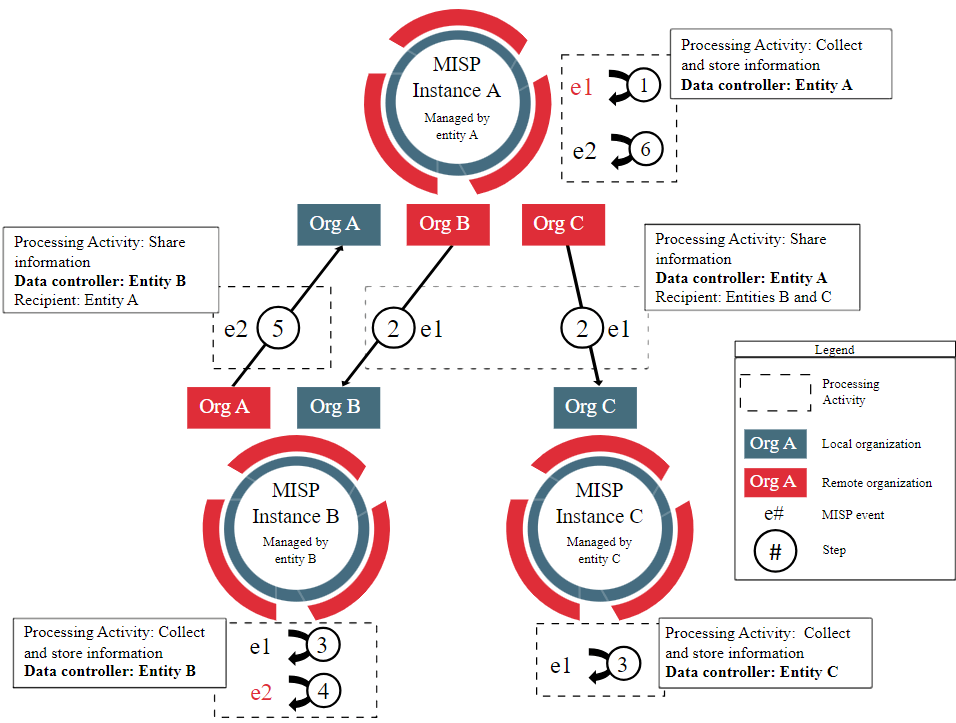
\includegraphics[width=0.8\textwidth]{assets/misp-compliance-gdpr.png}
    \caption[Démonstration de l'échange d'informations entre entités via MISP (source: \href{https://www.misp-project.org/compliance/GDPR/}{www.misp-project.org})]{Démonstration de l'échange d'informations entre entités via MISP}\label{fig:misp-compliance-gdpr}
\end{figure}

\vspace{1em}

\begin{itemize}[itemsep=0.8em]
    \item[•] \textbf{1 :} Un événement MISP "\textbf{e1}" est créé par l'entité \textbf{A}.
    \item[•] \textbf{2 :} L'entité \textbf{A} décide de partager l'événement avec des organisations distantes partenaires (entités \textbf{B} et \textbf{C}).
    \item[•] \textbf{3 :} Les entités \textbf{B} et \textbf{C} stockent l'événement "\textbf{e1}" dans leur instance locale de MISP.
    \item[•] \textbf{4 :} L'entité \textbf{B} crée un second événement "\textbf{e2}".
    \item[•] \textbf{5 :} L'entité \textbf{B} décide de ne partager "\textbf{e2}" qu'avec l'entité \textbf{A}.
    \item[•] \textbf{6 :} L'entité \textbf{A} stocke l'événement "\textbf{e2}".\\
\end{itemize}

\newpage

\label{chap3:mispEvents}
Un événement MISP est un ensemble structuré d'informations relatives à un incident, une menace ou une observation spécifique en matière de cybersécurité, qui est géré au sein de la plateforme MISP. Ces événements permettent d'organiser et de partager des informations détaillées sur divers types de cybermenaces, notamment les attaques de logiciels malveillants, les tentatives d'hameçonnage, les vulnérabilités et d'autres incidents de sécurité. Chaque événement MISP peut inclure plusieurs attributs et indicateurs de compromission (IOC) qui permettent de comprendre la menace et d'être capable de la détecter à nouveau. Un événement MISP se compose principalement des éléments suivants :\\

\begin{itemize}[itemsep=1em]
    \item[•] \textbf{\textit{Attributes} :} Il s'agit de données individuelles qui décrivent des caractéristiques spécifiques de l'événement. Les attributs peuvent inclure des adresses IP, des noms de domaine, des hachages de fichiers, des adresses électroniques, des URL, des échantillons de logiciels malveillants et d'autres détails techniques qui permettent d'identifier et d'analyser la menace.
    \item[•] \textbf{\textit{Tags} :} Les "Tags" sont utilisés pour classer et étiqueter les événements afin de faciliter la recherche et le filtrage. Les étiquettes peuvent inclure des classifications telles que "phishing", "APT" (Advanced Persistent Threat), "malware" ou "ransomware", ainsi que des informations sur la sensibilité ou les exigences de traitement des données.
    \item[•] \textbf{\textit{Objects} :} Ce sont des groupes d'attributs liés qui, ensemble, décrivent des entités ou des scénarios plus complexes, tels qu'une personne, un courrier électronique ou un périphérique de réseau. Cela permet de fournir un contexte et une structure aux données.
    \item[•] \textbf{\textit{Relations }:} Les événements peuvent être liés à d'autres événements ou objets pour indiquer les relations entre différents incidents, ce qui permet aux utilisateurs de voir les connexions et les corrélations qui ne sont pas toujours évidentes.
    \item[•] \textbf{\textit{Comments }:} Les utilisateurs peuvent ajouter des commentaires à un événement pour fournir un contexte, une analyse ou des recommandations supplémentaires, ce qui facilite la collaboration et le partage des connaissances entre les analystes.
    \item[•] \textbf{\textit{Threat Level/Analysis} :} Les événements comprennent souvent un indicateur de niveau de menace et de niveau d'avancement de l'analyse de l'événement (faible, moyen, élevé), qui peut aider à hiérarchiser la réponse à des menaces spécifiques.\\
\end{itemize}

\newpage

\begin{figure}[h]%
    \center%
    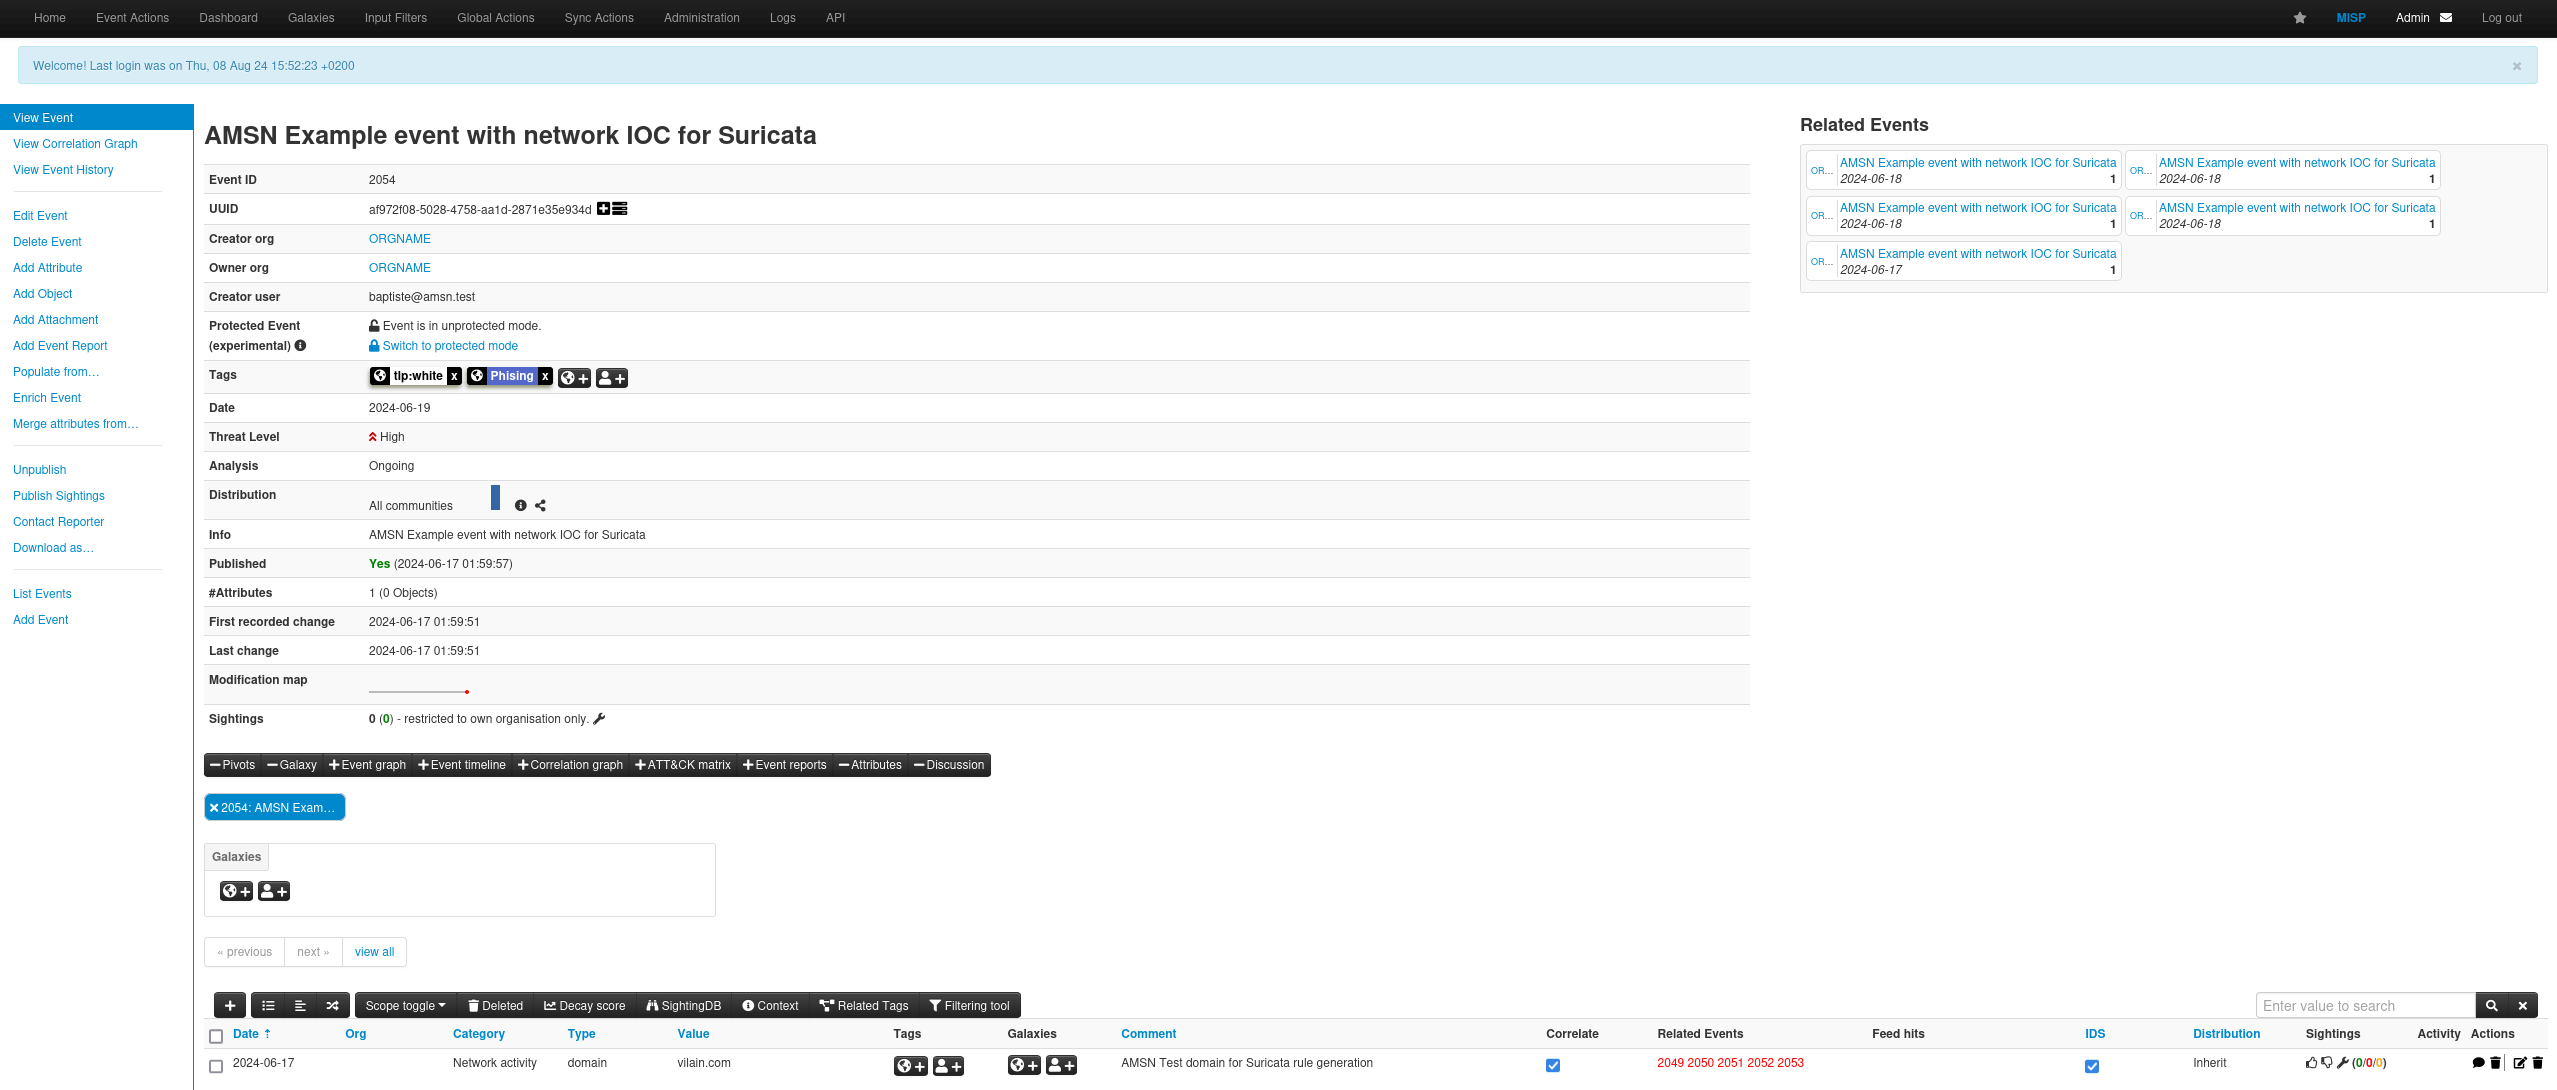
\includegraphics[width=1\textwidth]{assets/CaptureMisp.png}
    \caption[Exemple d'événement MISP (source : capture d'écran de l'interface graphique de l'instance de test locale MISP)]{Exemple d'événement MISP (source : capture d'écran de l'interface graphique de l'instance de test locale MISP)}\label{fig:CaptureMisp}
\end{figure}

\vspace{1em}

Parmi ces éléments, les plus importants pour répondre à notre problématique sont les \textit{Attributes} et les \textit{Objects} (qui sont des ensembles d'\textit{Attributes}), lesquels contiennent les éléments d'identification uniques des événements qui peuvent être utilisés pour créer des IOC, les autres servant principalement d'éléments de contexte et d'explication de l'événement. Dans ces \textit{Attributes}, je vais extraire les IOC compatibles avec Suricata (adresses IP, noms de domaine, URL, hachages de fichiers et User-Agent), afin de les transformer automatiquement en règles de détection qui seront ajoutées à notre ensemble de règles envoyées aux sondes.\\

\subsubsection{\textit{Note}}
J'ai également eu l'occasion d'effectuer quelques tâches supplémentaires avec MISP afin de soutenir le SOC-MC au quotidien. Les analystes du SOC m'avaient fait part de leur difficulté à comprendre certaines règles envoyées sans contexte par les partenaires. MISP m'a permis de répondre en partie à cette difficulté en offrant la possibilité de contextualiser les règles qui génèrent des alertes à partir d'événements sur le MISP partageant les mêmes IOC. Cependant, ce travail sort du cadre de ma problématique, voire est négligeable par rapport à l'ensemble de mon travail, je n'y reviendrai donc pas dans la suite de ce document.

\newpage

\subsection{Exploitation de MISP}

\vspace{1em}

La première étape de l'intégration de MISP dans le processus de mise à jour des règles a consisté à installer une VM (machine virtuelle), dans le réseau interne de l'Agence, à l'aide des guides fournis par le CIRCL\footnote{\url{https://misp.github.io/MISP/}}. Pour la tenir à jour avec les derniers événements partagés sur le réseau MISP sans avoir à exposer notre instance locale, j'ai utilisé MISP Guard\footnote{un addon mitmproxy développé par l'équipe qui est à l'origine de MISP : \url{https://www.misp-project.org/2022/09/13/misp-guard.html/}} qui permet de créer un proxy capable de récupérer les mises à jour de manière sécurisée sans menacer notre instance locale ou notre réseau interne.\\

\vspace{1em}

\begin{figure}[h]%
    \center%
    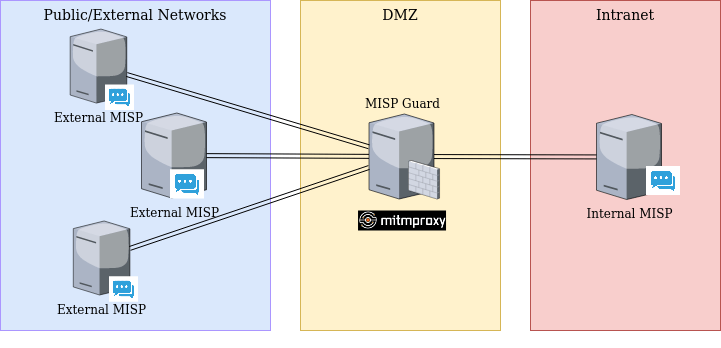
\includegraphics[width=0.85\textwidth]{assets/MispGard.png}
    \caption[Installation sécurisée de MISP dans le réseau de l'Agence (source: \url{https://www.misp-project.org/img/blog/misp-guard-architecture.png})]{Installation sécurisée de MISP dans le réseau de l'Agence}\label{fig:MispGard}
\end{figure}

L'instance locale de MISP est utilisée systématiquement via l'API. Mon travail sur le MISP a alors principalement consisté à développer des scripts Python utilisant PyMISP\footnote{\url{https://github.com/MISP/PyMISP}}, une bibliothèque Python open-source officielle du CIRCL qui facilite l'utilisation d'une instance locale du MISP. Mon travail de développement a été divisé en trois parties :\\

\begin{itemize}[itemsep=0.75em]
    \item[•] 1. Enrichissement de l'instance locale avec des IOC ;
    \item[•] 2. Sélection des IOC ;
    \item[•] 3. Génération de règles à partir des IOC.\\
\end{itemize}

\newpage

\subsubsection{Enrichissement de l'instance locale avec des IOC}
\vspace{0.5em}

La première étape pour rendre MISP utile après l'installation est de centraliser les données de renseignements à l'aide de l'API. Pour ce faire, j'ai développé un script dont la fonction est d'alimenter notre instance locale avec des événements provenant de sources publiques, d'une part, et de nos propres sources internes, d'autre part.\\

\vspace{1em}

\begin{figure}[h]%
    \center%
    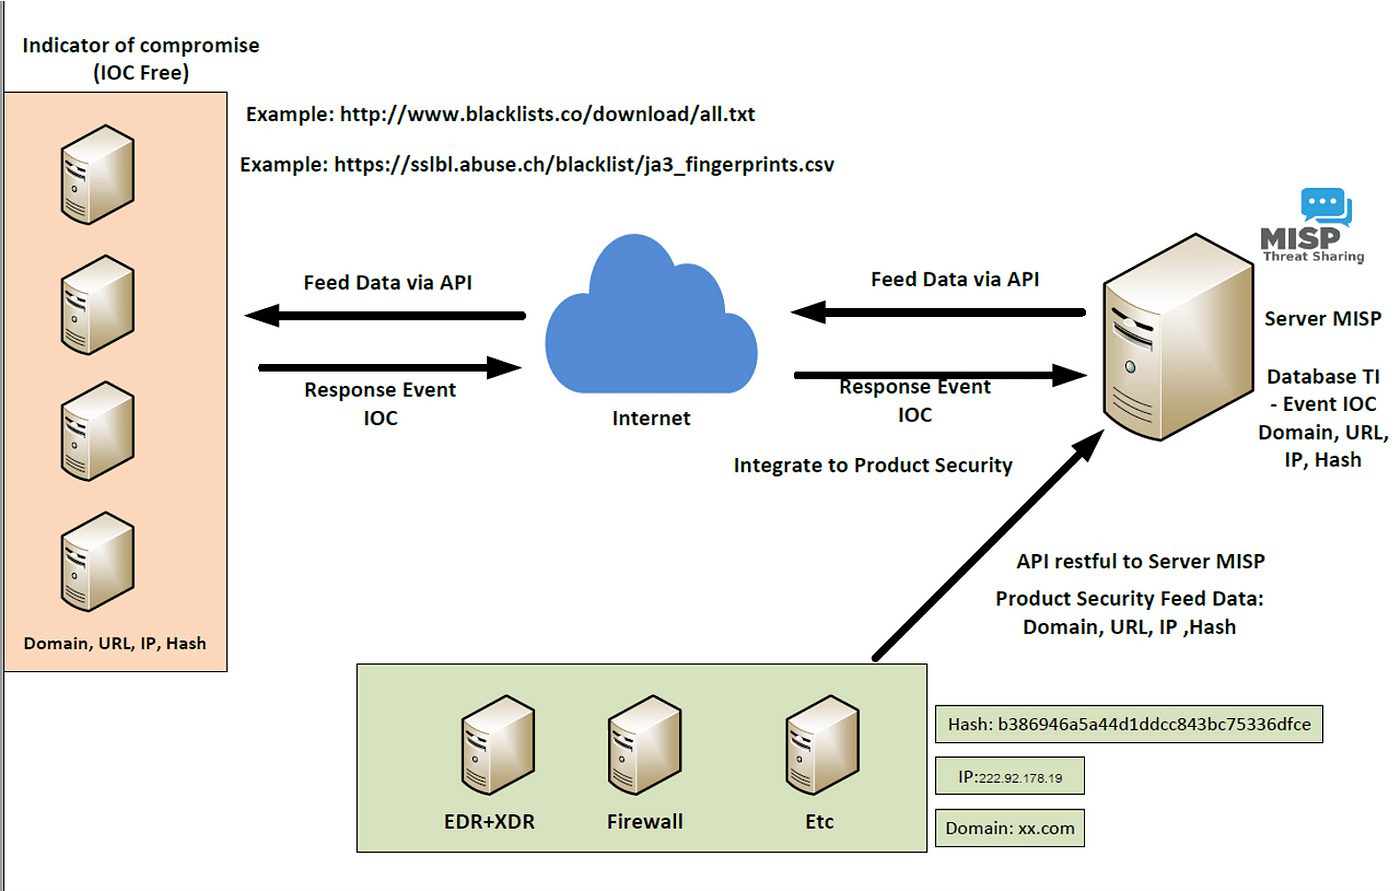
\includegraphics[width=0.9\textwidth]{assets/MispInfo.png}
    \caption[Récupération des IOC via l'API de notre instance MISP locale (source: \url{https://so-sonajaa.medium.com/misp-malware-information-sharing-platform-ep1-eea91df7415b})]{Récupération des IOC via l'API de notre instance MISP locale}\label{fig:MispInfo}
\end{figure}

\vspace{1em}

En ce qui concerne les sources publiques, si je n'ai utilisé que les deux "Feeds" fournis par défaut par le CIRCL\footnote{\url{https://www.circl.lu/doc/misp/feed-osint/}}\footnote{\url{https://www.botvrij.eu/data/feed-osint/}} lors de l'installation de l'instance, le travail que j'ai effectué permettra cependant l'intégration de sources supplémentaires à l'avenir.

\newpage

\begin{figure}[h]%
    \center%
\begin{lstlisting}[language=Python]
# Import PyMISP
from pymisp import PyMISP
# local misp credential
from conf.misp_conf import misp_url, misp_user_key, misp_verifycert

# source d'events "feeds" :
feeds = [
    "https://www.circl.lu/doc/misp/feed-osint/",
    "http://www.botvrij.eu/data/feed-osint/"
]
# Autres "feeds" potentiels :
#   "https://bazaar.abuse.ch/downloads/misp/",
#   "https://urlhaus.abuse.ch/downloads/misp/",
#   "https://osint.digitalside.it/Threat-Intel/digitalside-misp-feed/",

# Connexion avec l'instance MISP
misp = PyMISP(misp_url, misp_user_key, misp_verifycert, 'json')

# Recuperation des events depuis les "feeds"
download_events(feeds)

# Integration des events dans l'instance local MISP
import_events(misp)
\end{lstlisting}
{\small
    \textit{Télécharge les événements à partir des sources fournies et les importe dans notre instance locale. "download\_events(feeds)" la fonction qui télécharge les événements. "import\_events(misp)" celle qui les importe dans notre instance locale de MISP. \hyperref[chap:annexe3]{[A.3]}}
    }
    \caption[Enrichissement de l’instance locale de MISP en évènement]{Enrichissement de l’instance locale de MISP en évènement}\label{fig:GetEventsMISP}
\end{figure}

\vspace{1em}

La seule importation des évènements, publiés par ces deux sources au cours des années 2023 et 2024, suffit à remplir notre instance de dizaine de milliers d'événements pouvant chacun partager des centaines d'IOC.\\

En plus de ces événements, je récupère les IOC détectés par nos propres équipements (Firewall, Sonde, etc.) ou par nos partenaires et un autre script Python permet la transformation de ceux-ci en évènement MISP.\\

\newpage

\begin{figure}[h]%
    \center%
\begin{lstlisting}[language=Python]
# Import PyMISP et MISPEvent
from pymisp import PyMISP
# local misp credential
from conf.misp_conf import misp_url, misp_user_key, misp_verifycert

# Connexion avec l'instance MISP
misp = PyMISP(misp_url, misp_user_key, misp_verifycert, 'json')
event = MISPEvent()

# Creer un evenement sur l'instance local MISP
response = create_event(3, 1, 1, "AMSN Example event with network IOC for Suricata", {"category": 'Network activity', "type": 'domain', "value": 'Vilain.com', "comment": 'AMSN Test domain for Suricata rule generation'}, ["tlp:white", "Phising"])
\end{lstlisting}
{\small
   \textit{Créer un événement exploitable à partir des informations associées. "create\_event(...)" la fonction qui crée un événement à partir d'information fournie. \hyperref[chap:annexe3]{[A.3]}}
    }
    \caption[Création événement MISP]{Création événement MISP}\label{fig:CreateMispEvent}
\end{figure}

\vspace{1em}

Les événements créés et les informations qui y sont enregistrées ont été conçus pour être compréhensibles par les analystes du SOC-MC et pour être exportables sous la forme de règles Suricata de la même manière que \hyperref[chap3:genRulesEvents]{\textbf{\textit{les autres IOC}}}.

\newpage

\subsubsection{Sélection des IOC}
\vspace{0.5em}

\hyperref[chap3:mispEvents]{\textit{\textbf{Comme mentionné plus haut}}}, seule une minorité d'IOC peut être utilisée, en raison du choix des technologies de détection de l'Agence. Afin d'optimiser le poids de notre instance locale et sa vitesse de réaction aux requêtes API de mes scripts, j'ai créé un autre script qui nettoie automatiquement notre instance de tous les IOC que nous ne sommes pas en mesure d'utiliser.\\

\begin{figure}[h]%
    \center%
\begin{lstlisting}[language=Python]
# Import PyMISP et MISPEvent
from pymisp import PyMISP
# local misp credential
from conf.misp_conf import misp_url, misp_user_key, misp_verifycert

# Types d'IOC dont nous avons besoin
suricata_types = [
    'ip-dst', 'ip-src', 'domain', 'domain|ip', 'url', 'uri', 'hostname',
    'md5', 'sha1', 'sha256', 'sha512'
]

# Recuperation de tous les events de l'instance local
events = misp.search(controller='events')

# Interrogation des events et suppression des attributs incompatibles avec les donnees de Suricata
for event in events:
    event_id = event['Event']['id']
    misp_event = misp.get_event(event_id)
    
    for attribute in misp_event['Event']['Attribute']:
        if not is_suricata_compatible(attribute):
            # Suppression de l'attribut non compatible avec Suricata
            misp.delete_attribute(attribute['id'])
\end{lstlisting}
{\small
    \textit{Supprime tous les IOC qui ne font pas partie de ceux désignés dans la liste 'suricata\_types' de l'instance local MISP.}
    }
    \caption[Suppression des IOC inutiles]{Suppression des IOC inutiles}\label{fig:RemoveIOC}
\end{figure}

\vspace{1em}

En outre, j'utilise une fonctionnalité offerte par MISP, les "Decaying Models"\footnote{\url{https://www.misp-project.org/2019/09/12/Decaying-Of-Indicators.html/}} qui attribuent aux IOC une durée de vie en fonction de leur type et un score qui diminue au fil du temps.\\

\newpage

\begin{figure}[h]%
    \center%
    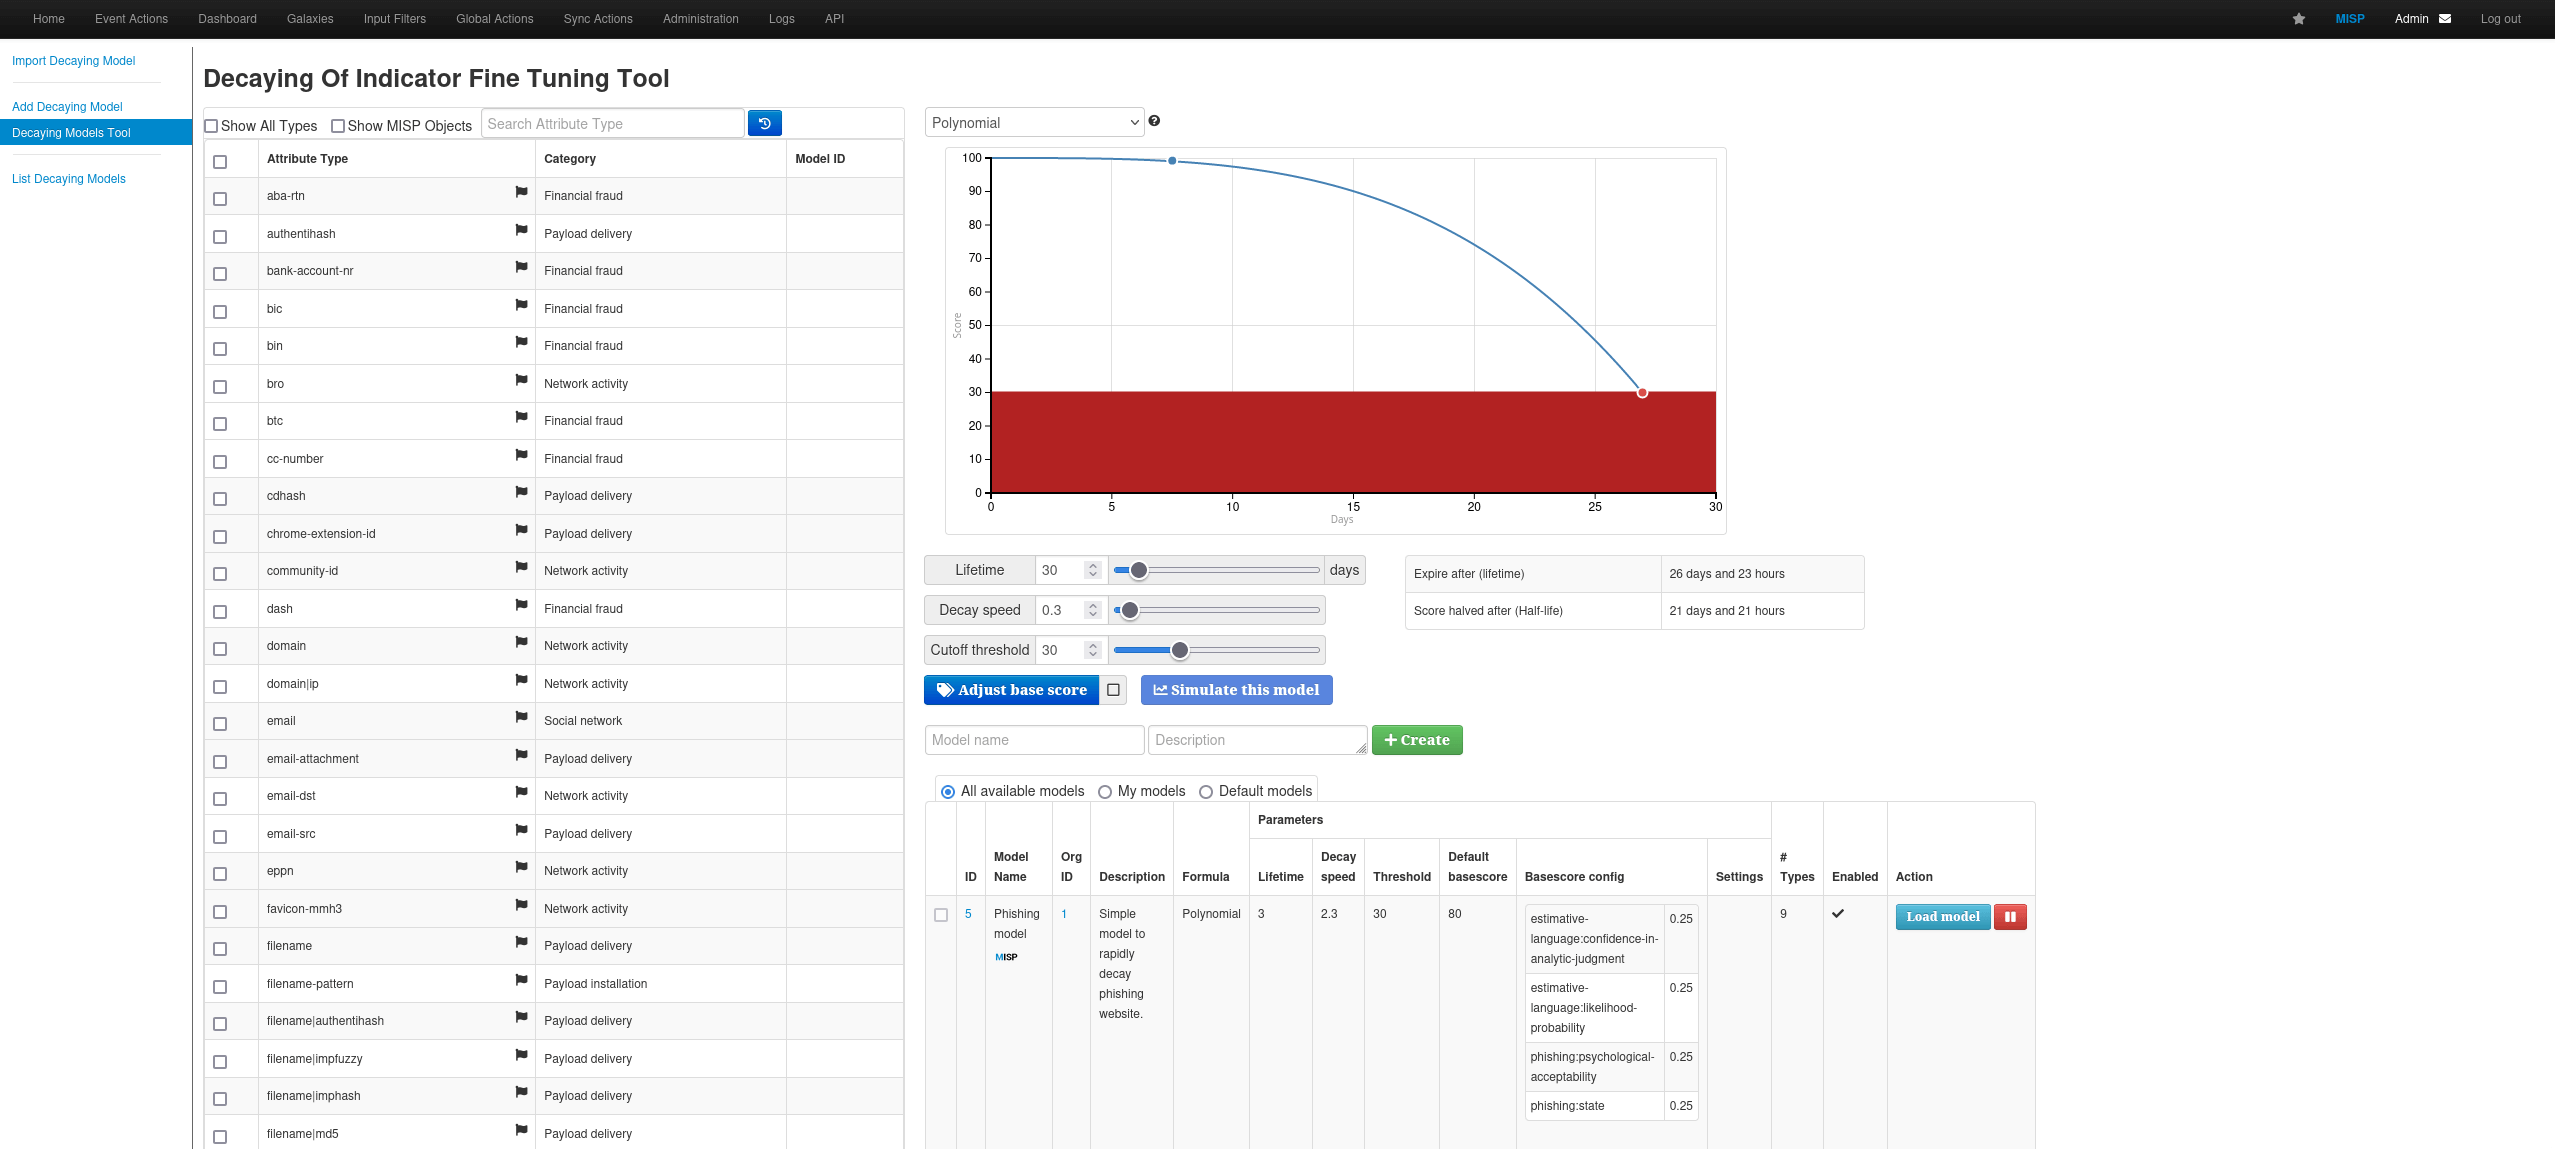
\includegraphics[width=1\textwidth]{assets/CaptureDecayingModel.png}
    \caption[Exemple de "Decaying Model" (source : capture d'écran de l'interface graphique de l'instance de test locale MISP)]{Exemple de "Decaying Models" (source : capture d'écran de l'interface graphique de l'instance de test locale MISP)}\label{fig:CaptureDecayingModel}
\end{figure}

\vspace{1em}

Pour l'instant, le modèle par défaut proposé par le MISP "NIDS Simple Decaying Model"\footnote{\url{https://github.com/MISP/misp-decaying-models/blob/main/models/nids-simple-model.json}} est utilisé sur l'instance. Les adresses IP, les noms de domaine et les URL ont ainsi une durée de vie de deux mois, après quoi les IOC en question sont considérés comme obsolètes (car la probabilité que ces IOC ne soient plus utilisés, par les acteurs malveillants détectés à l'origine, est trop élevée). \hyperref[biblio]{[2]}\\

À terme, l'AMSN souhaiterait travailler à la création de ses propres modèles d'obsolescence des IOC sur la base du retour d'information des analystes du SOC-MC et de ses partenaires.

\newpage

\subsubsection{Génération de règles à partir des IOC}
\label{chap3:genRulesEvents}
\vspace{0.5em}

Une fois que l'instance locale a été remplie d'événements et que les données ont été nettoyées, PyMISP offre la possibilité d'exporter directement les \textit{Attributes} des événements en règles Suricata.\\

\vspace{1em}

\begin{figure}[h]%
    \center%
\begin{lstlisting}[language=Python]
# Import PyMISP et MISPEvent
from pymisp import PyMISP
# local misp credential
from conf.misp_conf import misp_url, misp_user_key, misp_verifycert

# Prend tous les events et fabrique avec un fichier .rules exploitable
suricata_rules = misp.search(controller='events', return_format="suricata")
\end{lstlisting}
{\small
    \textit{Génère des règles de suricata à partir des IOC de tous les événements présents dans l'instance locale.}
    }
    \caption[Génération de règle Suricata depuis l'instance local MISP]{Génération de règle suricata depuis l'instance local MISP}\label{fig:CreateSuricataMISP}
\end{figure}

\vspace{1em}

Pour chaque attribut d'événement, une règle Suricata capable de détecter l'IOC de l'attribut est générée. Par exemple :\\

\newpage

\begin{figure}[h]%
    \center%
    L'IOC :\\
    \vspace{0.5em}
    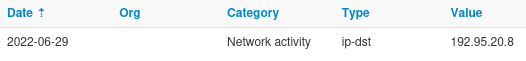
\includegraphics[width=0.9\textwidth]{assets/IP.png}
    \vspace{1em}
    \\Provenant de l'évènement :\\
    \vspace{0.5em}
    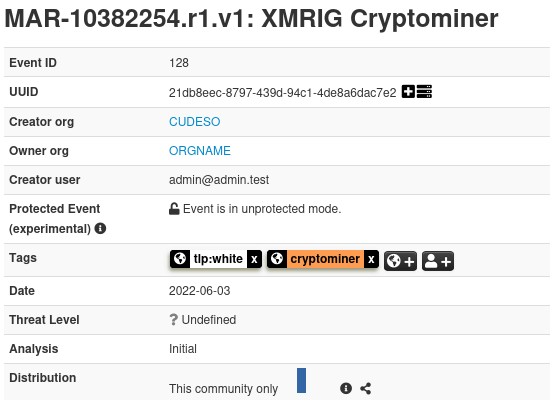
\includegraphics[width=0.8\textwidth]{assets/MispEventRule.png}
    \vspace{1em}
    \\Génère la règle :
    \begin{lstlisting}[language=bash]
alert ip $HOME_NET any -> 192.95.20.8 any (msg: "MISP e128 [] Outgoing To IP: 192.95.20.8"; classtype:trojan-activity; sid:2696602; rev:1; priority:4; reference:url,https://192.168.215.128/events/view/128;)
\end{lstlisting}
    
    \caption[Exemple de génération de règle Suricata par MISP (source : capture d'écran de l'interface graphique de l'instance de test locale MISP)]{Exemple de génération de règle Suricata par MISP (source : capture d'écran de l'interface graphique de l'instance de test locale MISP)}\label{fig:IP}
\end{figure}

\vspace{1em}

Les tests effectués avec le SOC-MC ont révélé que ces règles étaient fonctionnelles en l'état, mais qu'elles ne contenaient pas les informations contextuelles nécessaires pour comprendre et classer les alertes qu'elles généraient. Cela m'a conduit à créer un script supplémentaire pour reformater les règles générées par MISP. Pour ce faire, je n'ai modifié que deux variables dans la section \textit{options} des règles qui n'affectent pas leur capacité de détection :\\

\newpage

\begin{itemize}[itemsep=1em]
    \item[•] Soit la variable 'msg' (qui est une variable facultative utilisée pour donner des informations contextuelles sur la règle) en indiquant le nom de l'événement lié à la règle avec un lien vers l'événement sur l'interface graphique de l'instance MISP, à laquelle les analystes SOC peuvent accéder depuis leur poste de travail à l'aide de leur navigateur ;
    \item[•] Et la variable 'metadata' (qui est une variable optionnelle utilisée pour donner des informations supplémentaires à une règle) que j'ai complétée pour ajouter les 'Tags' de l'événement lié à cette règle.\\
\end{itemize}

\begin{figure}[h]%
    \center%
\begin{lstlisting}[language=Python]
# Prend tous les events
suricata_rules = misp.search(controller='events', return_format="suricata")

for rule in suricata_rules:
    ruleurl = re.search(r'reference:url,(.*?);', rule)
    if ruleurl:
        # On remplace le message original des regles (peu lisible et trop long) par un message simple renvoyant vers la pages MISP de l'Event
        rule = re.sub(r'msg: "(.*?)";', 'msg: "MISP event: ' + ruleurl.group(1) + '";', rule)
        # Ajout des tags de l'events
        rule = re.sub(r'metadata: "(.*?)";', 'metadata: tags ' + eventTags + '";', rule)
        new_lines.append('alert ' + rule)
\end{lstlisting}
{\small
    \textit{Modifie les variables des règles générées par MISP.}
}

\vspace{1em}
Règle après modifications :
\vspace{0.5em}
\begin{lstlisting}[language=bash]
alert ip $HOME_NET any -> 192.95.20.8 any (msg: "MISP Event : MAR-10382254.r1.v1: XMRIG Cryptominer https://192.168.215.128/events/view/128"; classtype:trojan-activity; sid:2696602; rev:1; priority:4; reference:url,https://192.168.215.128/events/view/128; metadata: tags tlp:white|cryptominer;)
\end{lstlisting}
    \caption[Modification des règles générées par MISP]{Modification des règles générées par MISP}\label{fig:ModifRulesMISP}
\end{figure}

\vspace{1em}

L'ajout du titre de l'événement présente l'avantage d'indiquer plus clairement aux analystes l'objectif de détection de la règle, et le lien vers l'interface graphique MISP leur permet de rechercher plus d'informations sur la règle directement sur MISP en cas d'investigation.\\ 

\newpage

L'ajout de "Tags" à l'événement fournit également des informations supplémentaires sur la règle, mais permet surtout de classer les règles en catégories, qui peuvent ensuite être utilisées pour créer des statistiques basées sur celles-ci, ou évaluer leur utilité en fonction des sondes sur lesquelles elles seront appliquées.\\

Une fois reformatées, les règles générées peuvent être directement ajoutées aux règles ingérées par \hyperref[chap3:section1]{\textbf{\textit{mon premier programme}}} pour être intégrées dans les sondes.

\vspace{1em}

\subsubsection{\textit{Note}}
Le développement de ce code a également pris environ un mois et demi, comprenant la rédaction de la documentation. L'instance de MISP mentionnée dans cette section a été installée et testée dans une section distincte du réseau interne avec des données de test. Les réactions de mon tuteur de stage et des analystes du SOC-MC sont positives quant au potentiel offert par cette instance locale, mais pour l'instant, elle n'est pas encore utilisée dans les processus actuels de l'Agence, dans l'attente de la planification du déplacement de la VM de l'instance sur le réseau de production.
}

\newpage

\section{Filtrage des règles générées par OIV}
\label{chap3:section3}
{\fontsize{14pt}{16pt}\selectfont
    %%%%%%%%%%%%%%%%%%%%%%%%%%%%
% SECTION                  %
%%%%%%%%%%%%%%%%%%%%%%%%%%%%
\vspace{1em}

Un dilemme s'est posé lors de l'ajout des règles de MISP à celles des partenaires. Le nombre total de règles ingérées par les sondes se comptait auparavant en dizaine de milliers, mais une fois les règles MISP ajoutées, ce nombre s'élevait à des centaines de milliers.\\

\vspace{1em}

\begin{figure}[h]%
    \center%
    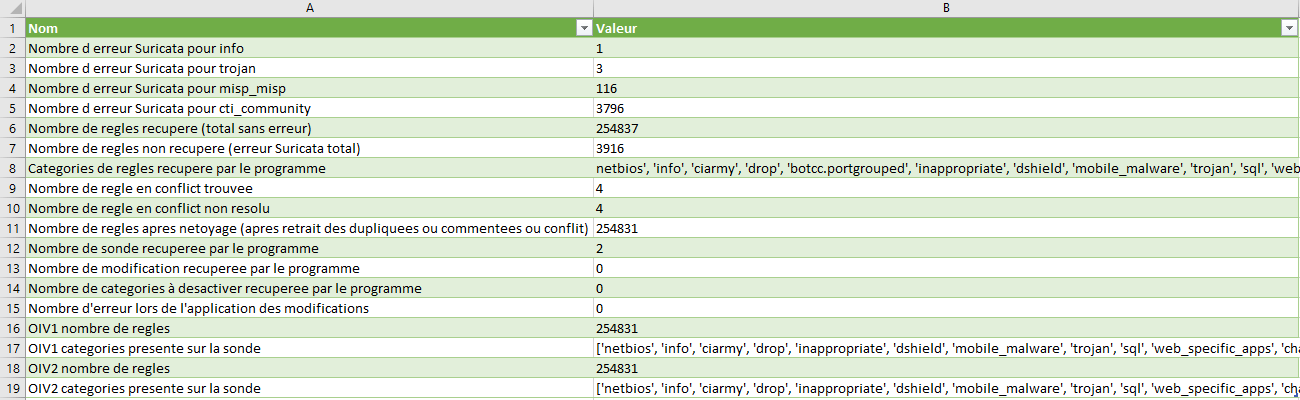
\includegraphics[width=1
    \textwidth]{assets/statMISP.png}
    \caption[Fichier CSV des statistique du programme après intégration des règles provenant de MISP]{Fichier CSV des statistique du programme après intégration des règles provenant de MISP}\label{fig:statMISP}
\end{figure}

\vspace{1em}

Ce nombre très élevé de règles risque de surcharger les sondes et de les ralentir, ce qui serait préjudiciable aux réseaux sur lesquels elles sont installées.\\

De plus, l'implémention de centaines de milliers de règles sans filtrage des sondes augmente considérablement le risque d'avoir des règles inutiles ou de provoquer de nombreux faux positifs (détection erronée d'une menace ou d'une activité malveillante par un système de sécurité) qui peuvent surcharger les équipes de sécurité de l'Agence. Un véritable défi se  pose alors pour filtrer les règles en fonction des OIV afin de maximiser leur efficacité et d'optimiser le nombre de règles appliquées à chaque sonde.\\

\newpage

 J'ai pu travailler sur ce point conjointement avec les membres du SOC-MC afin de hiérarchiser les règles en fonction de leur source et de leur type pour chaque OIV. D'une part, les règles fournies par les partenaires de renseignement sont classées en fonction de leur rôle et certaines d'entre elles sont destinées à des technologies spécifiques (par exemple 'SQL', 'ACTIVEX', 'SCADA', etc.). D'autre part dans l'environnement MISP, il est possible d'utiliser la fonctionnalité 'Tags' des événements pour trier les règles en catégories (par exemple les tags 'linux', 'windows', 'javascript', 'HealthCare', etc.).\\

En établissant ces catégories, nous pouvons ensuite, grâce à notre connaissance des technologies présentes sur les réseaux des OIV et leur collaboration avec l'Agence, estimer les règles pertinentes à retenir sur chaque sonde. Pour ce faire, j'ai complété \hyperref[chap3:section1]{\textbf{\textit{mon programme de gestion des règles}}} en ajoutant un segment permettant de désactiver des ensembles de règles en fonction de leur catégorie.\\

Ce nouveau segment fonctionne exactement comme \hyperref[chap3:section1rulesmodif]{\textbf{\textit{la section de modifications des règles}}}, mais utilise un autre fichier CSV fourni pour sélectionner les catégories de règles à supprimer pour les sondes.\\

\vspace{1em}

\begin{figure}[h]%
    \center%
    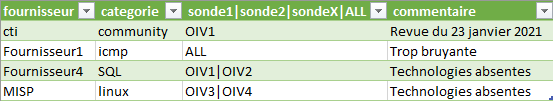
\includegraphics[width=0.8\textwidth]{assets/CategoriDisable.png}
    \caption[Exemple de fichier CSV de contrôle des catégories de règles]{Exemple de fichier CSV de contrôle des catégories de règles}\label{fig:CategoriDisable}
\end{figure}

\vspace{0.5em}

\begin{figure}[h]%
    \center%
\begin{lstlisting}[language=Python].
# Fonction pour parcourir les regles des sondes pour faire si possible la modification
def disable_categories(rulesByProbes, SelectedSondes, categorie, toDisable, modification_error):
    # On parcourt chaque sondes cible
    for sonde in SelectedSondes:
        # On cherche si la categorie existe dans la sonde cible
        if (categorie in rulesByProbes[sonde[0]]["source"].tolist()):
            targetRow = rulesByProbes[sonde[0]][rulesByProbes[sonde[0]]["source"].str.contains(categorie)]
            rulesByProbes[sonde[0]] = rulesByProbes[sonde[0]].drop(targetRow.index)
\end{lstlisting}
{\small
    \textit{Supprime les règles appartenant à certaines catégories sur des sondes ciblées.}
}
\caption[Contrôle des catégories sur les sondes]{Contrôle des catégories sur les sondes}\label{fig:RemoveCategorie}
\end{figure}

\newpage

Ce code ajouté permet de supprimer des milliers de règles ciblées sur chaque sonde, en ne conservant que celles qui sont les plus pertinentes, réduisant le nombre de règles par sonde à des niveaux plus supportables.

\vspace{1em}

\begin{figure}[h]%
    \center%
    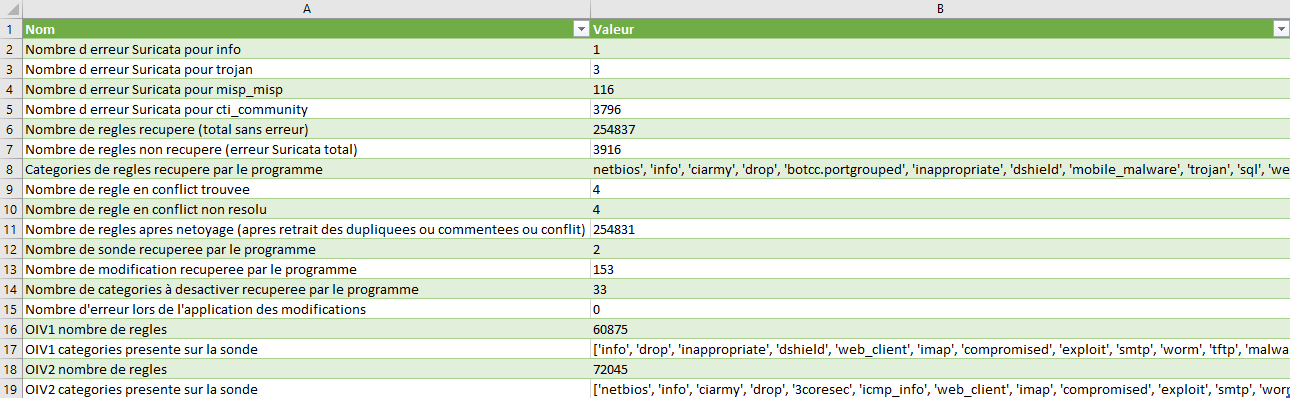
\includegraphics[width=1
    \textwidth]{assets/statOpti.png}
    \caption[Fichier CSV des statistiques du programme après sélection des catégories par sonde]{Fichier CSV des statistiques du programme après sélection des catégories par sonde}\label{fig:CategoriStat}
\end{figure}

\vspace{1em}

\subsubsection{\textit{Note}}
Cette partie s'est déroulée sur quelques semaines, incluant la complétion de la documentation réalisée précédemment avec les nouveaux changements. Ensuite, le temps restant de mon stage a été consacré à la rédaction de ma thèse professionnelle, à sa relecture et à sa correction en collaboration avec mon tuteur de stage.
}

\chapter{Résultat}%
\label{chap:4}
%%%%%%%%%%%%%%%%%%%%%%%%%%%%
% CHAPTER                  %
%%%%%%%%%%%%%%%%%%%%%%%%%%%%

\section{Analyse des résultats}
\label{chap4:section1}
{\fontsize{14pt}{16pt}\selectfont
    %%%%%%%%%%%%%%%%%%%%%%%%%%%%
% SECTION                  %
%%%%%%%%%%%%%%%%%%%%%%%%%%%%
\vspace{1em}

La gestion des sondes de détection peut être perçue comme une tâche complexe et contraignante pour les organisations impliquées dans la supervision des réseaux. Alors que les solutions proposées par des sociétés privées sont souvent très coûteuses, mon travail a permis de créer un outil interne facilitant le travail quotidien des membres du CERT-MC. Le \hyperref[chap3:intro]{\textit{\textbf{processus de gestion des sondes}}} de l'Agence a ainsi pu recevoir les améliorations suivantes:\\

\vspace{1em}

\begin{itemize}[itemsep=1em]
    \item[•] Les règles envoyées aux sondes sont désormais contrôlées avant d'être utilisées, minimisant ainsi le risque d’erreurs au moment du déploiement sur les sondes ;
    \item[•] Il est maintenant possible de désactiver ou de modifier des règles spécifiques parmi celles envoyées aux sondes, offrant une meilleure flexibilité dans leur gestion ;
    \item[•] Les règles provenant de MISP peuvent désormais être intégrées directement dans les sondes, enrichissant ainsi les sources d’informations pour une meilleure détection des menaces ;
    \item[•] Les règles sont catégorisées, et il est possible de désactiver certaines catégories en fonction des besoins spécifiques de chaque sonde.\\
\end{itemize}

\newpage

Ces améliorations ont considérablement optimisé le processus d'alimentation des sondes de l'Agence.  En particulier, la possibilité de filtrer et d'ajuster dynamiquement les règles réduit les faux positifs, minimise la surcharge du système et facilite le travail des analystes du SOC-MC en leur fournissant un outil simple de gestion des règles.\\

A l'avenir, l'AMSN souhaite poursuivre le développement de l'outil, notamment son interfaçage avec MISP, afin d'étendre les capacités de détection de l'Agence par l'ajout de nouveaux flux d'information. Le dilemme de l'optimisation des règles, présentes sur les sondes, continuera à se poser et nécessitera un renforcement des relations entre l'Agence et ses OIV pour une meilleure sélection des catégories dont ils relèvent.
}

\newpage

\section{Bilan personnel}
\label{chap4:section2}
{\fontsize{14pt}{16pt}\selectfont
    %%%%%%%%%%%%%%%%%%%%%%%%%%%%
% SECTION                  %
%%%%%%%%%%%%%%%%%%%%%%%%%%%%
\vspace{1em}

Mon expérience au sein de l'Agence Monégasque de Sécurité Numérique fut très enrichissante, tant sur le plan technique que professionnel. Ce stage m'a introduit au monde de la cybersécurité Étatique. J'ai pu côtoyer pour la première fois un CERT national et être témoin de leurs missions et organisations au quotidien. Ou encore travailler sur des problématiques concrètes, développer des solutions adaptées à des enjeux réels, et contribuer de manière significative à l'amélioration des processus de l'Agence.\\

Le projet de développement d'un outil automatisé de génération de règles de détection m'a permis de m'immerger dans des technologies clés des IDS de Suricata et de MISP, tout en approfondissant mes connaissances en programmation, notamment avec Python. La résolution de problèmes complexes, comme la gestion de milliers de règles et l'optimisation de leur efficacité, a développé ma capacité à analyser des situations et à proposer des solutions techniques robustes.\\

Sur le plan personnel, cette expérience m'a enseigné à mieux structurer mon travail, à collaborer avec des équipes multidisciplinaires, et à gérer un projet de bout en bout, depuis l'analyse des besoins jusqu'à la mise en production. J'ai également beaucoup appris en termes de communication, notamment en partageant régulièrement mes avancées avec mon tuteur de stage et les analystes du SOC-MC.\\

Enfin, cette période a renforcé mon intérêt pour le domaine de la cybersécurité et m'a confirmé dans mon choix de carrière. J'ai non seulement acquis des compétences techniques et méthodologiques, mais aussi développé une meilleure compréhension des enjeux stratégiques liés à la protection des systèmes d'information. Mon passage à l'AMSN m'a donné confiance en mes capacités à mener des projets ambitieux et à contribuer activement à la sécurisation des infrastructures numériques.
}

\chapter*{Conclusion et Perspectives}
\label{chap:conclusion}
{\fontsize{14pt}{16pt}\selectfont
    \markboth{\MakeUppercase{Conclusion et Perspectives}}{}%
\addcontentsline{toc}{chapter}{Conclusion et Perspectives}%

Le développement d’un outil de gestion centralisée de règles de détection d’intrusion représente une étape clé dans l'amélioration de la réactivité et de la pertinence des systèmes de défense contre les cybermenaces. Ce document et le travail qu'il présente a permis d’apporter des solutions à une problématique complexe, tout en répondant aux exigences opérationnelles d’un organisme en charge de la protection des infrastructures critiques.\\

L'automatisation de la gestion des règles de détection permet non seulement de simplifier et d'accélérer les processus de mise à jour, mais aussi d’améliorer la précision et l’adaptabilité des systèmes de détection d’intrusion dans un contexte où les menaces évoluent rapidement. Ce projet a démontré l’importance de combiner des approches techniques pointues avec une vision stratégique, afin de mieux répondre aux enjeux de cybersécurité auxquels sont confrontés autant les États que les organisations.\\

Cependant, ce travail ne représente qu’une première étape dans l’évolution vers des systèmes de détection plus intelligents et plus proactifs. Les perspectives d’amélioration sont nombreuses. D’une part, une meilleure collaboration entre les différentes entités publiques et privées, à travers le partage accru de renseignements sur les menaces, est un progrès souhaitable pour renforcer l’efficience des systèmes de détection d'intrusion. D’autre part, l'optimisation des règles en fonction des spécificités des infrastructures surveillées constitue un axe de développement essentiel pour minimiser les faux positifs et maximiser l’efficacité des sondes.\\

En conclusion, ce projet de fin d’études a non seulement contribué à répondre à des problématiques techniques concrètes, mais il ouvre également la voie à des évolutions futures dans le contexte étudié. Le cheminement entrepris dans ce cadre est le reflet d’un besoin constant d’innovation et d’adaptation face à un environnement en perpétuelle mutation, où la sécurité des systèmes d’information demeure un enjeu de premier plan.\\
}

\chapter*{Glossaire}
\label{chap:glossaire}
\markboth{\MakeUppercase{Glossaire}}{}%
\addcontentsline{toc}{chapter}{Glossaire}%

\begin{table}[ht!]
    \centering
    \small
    \begin{tabularx}{\textwidth}{|X|X|}
        \hline
        \textbf{AMSN (Agence Monégasque de Sécurité Numérique)} & Autorité nationale de l'Etat de Monaco en charge de la sécurité des systèmes d’information et des infrastructures critiques nationales  \\
        \hline
        \textbf{ANSSI (Agence Nationale de la Sécurité des Systèmes d'Information)} & Organisme français chargé de la protection des systèmes d'information de l'État et des infrastructures critiques nationales \\
        \hline
        \textbf{API (Application Programming Interface)} & Ensemble de règles et de protocoles permettant à des applications ou services de communiquer entre eux \\
        \hline
        \textbf{CERT (Computer Emergency Response Team)} & Groupe de spécialistes formés et expérimentés dans le domaine de la réponse aux incidents de sécurité informatiques \\
        \hline
        \textbf{CIRCL (Computer Incident Response Center Luxembourg)} & Centre national luxembourgeois de réponse aux incidents de sécurité informatique \\
        \hline
        \textbf{CSV (Comma-Separated Values) } & Format de fichier texte où les données sont organisées en lignes et colonnes, chaque valeur étant séparée par une virgule ou un autre délimiteur \\
        \hline
        \textbf{CTI (Cyber Threat Intelligence)} & Collecte et analyse de données relatives aux cybermenaces pour anticiper, prévenir et répondre aux attaques \\
        \hline
        \textbf{IDS (Intrusion Detection System)} & Système de sécurité qui surveille le trafic réseau ou les activités système pour détecter des comportements suspects ou des intrusions \\
        \hline
        \textbf{IOC (Indicator of Compromise)} & Signe observable, tel qu'une adresse IP malveillante ou un fichier suspect, qui indique une potentielle compromission ou intrusion dans un système \\
        \hline
        \textbf{MISP (Malware Information Sharing Platform)} & Plateforme open-source dédiée au partage d'indicateurs de compromission et de renseignements sur les cybermenaces \\
        \hline
        \textbf{OIV (Opérateur d'Importance Vitale)} & Organisation identifiée par l'État comme ayant des activités indispensables à la survie de la nation ou dangereuses pour la population \\
        \hline
        \textbf{SOC (Security Operation Center)} & Équipe centralisée chargée de surveiller, détecter et répondre aux menaces de sécurité en temps réel au sein d'une organisation \\
        \hline
    \end{tabularx}
\end{table}

\newpage

\begin{table}[ht!]
    \centering
    \small
    \begin{tabularx}{\textwidth}{|X|X|}
        \hline
        \textbf{VM (Virtual Machine)} & Environnement informatique simulé qui émule un système physique complet, permettant d'exécuter un système d'exploitation et des applications de manière isolée \\
        \hline
    \end{tabularx}
\end{table}

\newpage
\appendix

\chapter*{Annexe}
\label{chap:Annexe}
%%%%%%%%%%%%%%%%%%%%%%%%%%%%
% Annexe                  %
%%%%%%%%%%%%%%%%%%%%%%%%%%%%
\markboth{\MakeUppercase{Annexe}}{}%
\addcontentsline{toc}{chapter}{Annexe}%

\section{configTestSuricata.yaml}
\label{chap:annexe1}

Fichier de configuration Suricata utilisé lors de test de fichier. Les fonctionnalités non exploitées sont désactivées ("enabled: no") et les autres fonctionnalités (non montrées ici) sont laissées avec leurs valeurs par défaut.

\vspace{1em}

\begin{figure}[h]%
    \center%
\begin{lstlisting}[language=Bash]
%YAML 1.1
---
# This configuration file generated by Suricata 7.0.3.
suricata-version: "7.0"
# The default logging directory.
default-log-dir: /var/log/suricata/
# Global stats configuration
stats:
  enabled: yes
  # The interval field (in seconds) controls the interval at
  # which stats are updated in the log.
  interval: 8
# Configure the type of alert (and other) logging you would like.
outputs:
  # a line based alerts log similar to Snort's fast.log
  - fast:
      enabled: no
      filename: fast.log
  # Extensible Event Format (nicknamed EVE) event log in JSON format
  - eve-log:
      enabled: no
      filename: eve.json
      xff:
        enabled: no
        mode: extra-data
        header: X-Forwarded-For
  # output module to store certificates chain to disk
  - tls-store:
      enabled: no
  # By default all packets are logged except:
  # - TCP streams beyond stream.reassembly.depth
  # - encrypted streams after the key exchange
  - pcap-log:
      enabled: no
\end{lstlisting}
\end{figure}

\newpage

\begin{figure}[h]%
    \center%
\begin{lstlisting}[language=Bash]
  # a full alert log containing much information for signature writers
  # or for investigating suspected false positives.
  - alert-debug:
      enabled: no
      filename: alert-debug.log
      append: yes
  # Stats.log contains data from various counters of the Suricata engine.
  - stats:
      enabled: no
      filename: stats.log
      append: yes
  # a line based alerts log similar to fast.log into syslog
  - syslog:
      enabled: no
      # reported identity to syslog. If omitted the program name (usually
      # suricata) will be used.
      facility: local5
# Logging configuration. This is not about logging IDS alerts/events, but
# output about what Suricata is doing, like startup messages, errors, etc.
logging:
  # The default log level:
  default-log-level: Notice
  # Define your logging outputs.
  outputs:
  - console:
      enabled: yes
      level: Error
  - file:
      enabled: yes
      level: Error
      filename: suricata.log
  - syslog:
      enabled: yes
      facility: local5
      format: "[%i] <%d> -- "
rule-files:
  - suricata.rules

...
\end{lstlisting}
\end{figure}

\newpage

\section{Résultat Test Suricata}
\label{chap:annexe2}

Journal généré lors de l'exécution des fichiers de règles récupérées par le programme Python. Pour chaque règle non fonctionnelle sur notre version de Suricata, une première ligne décrit l'erreur qui s'est produite et une seconde ligne donne la règle qui a causé l'erreur ainsi que son fichier et sa ligne source.

\vspace{1em}

\begin{figure}[h]%
    \center%
\begin{lstlisting}[language=Bash]
[2449438 - Suricata-Main] 2024-09-26 09:14:21 Error: detect-parse: "$HOME_NET" is not a valid direction modifier, "->" and "<>" are supported.
[2449438 - Suricata-Main] 2024-09-26 09:14:21 Error: detect: error parsing signature "alert tcp $EXTERNAL_NET $HTTP_PORTS-> $HOME_NET any (msg: "MISP event:https://10.0.37.3/events/view/430";flow:established,to_client; content:"// stop for sometime if needed"; classtype:trojan-activity;reference:url,https://10.0.37.3/events/view/430; rev:1; sid:10924794;)" from file rules/misp/misp.rules at line 69127
[2449438 - Suricata-Main] 2024-09-26 09:14:21 Error: detect-parse: bad option value formatting (possible missing semicolon) for keyword content: '"/4419d5733u64c64888l9223d5belafc887d0.html__'
[2449438 - Suricata-Main] 2024-09-26 09:14:21 Error: detect: error parsing signature "alert http $HOME_NET any -> $EXTERNAL_NET $HTTP_PORTS (msg: "MISP event:https://10.0.37.3/events/view/714"; flow:to_server,established; http.header; content:"notifyhubss.net"; fast_pattern; nocase; http.uri; content:"/4419d5733u64c64888l9223d5belafc887d0.html__;!!OepYZ6Q!6a0JnRhFyhQfncK-LhrwBwz4hNh8MS_qxKKgAFDPEKMOCOgQxgYx7CnrvR6bIX3SIR-AMI9IhS0nwyds8fRelwKk4eFibA$"; nocase; tag:session,600,seconds; classtype:trojan-activity; sid:11031604; rev:1; priority:2; reference:url,https://10.0.37.3/events/view/714;)" from file rules/misp/misp.rules at line 76469
[2449438 - Suricata-Main] 2024-09-26 09:14:23 Error: detect-sid: invalid character as arg to sid keyword
[2449438 - Suricata-Main] 2024-09-26 09:14:23 Error: detect: error parsing signature "alert tcp any any -> any any (msg: "MISP event:https://10.0.37.3/events/view/1278"; sid:XX; rev:1; flow:established,to_server; content:"Accept|3a 20 2a 2f 2a|"; nocase; content:"HX1|3a|"; distance:0; within:6; fast_pattern; content:"HX2|3a|"; nocase; distance:0; content:"HX3|3a|"; nocase; distance:0; content:"HX4|3a|"; nocase; distance:0; classtype:trojan-activity; priority:X; sid:11468464;reference:url,https://10.0.37.3/events/view/1278;)" from file rules/misp/misp.rules at line 106142
[2449438 - Suricata-Main] 2024-09-26 09:14:28 Error: suricata: Loading signatures failed.
...
\end{lstlisting}
\end{figure}

\newpage

\section{Fonctions MISP}
\label{chap:annexe3}
\begin{figure}[h]%
    \center%
\begin{lstlisting}[language=Python].
# Telechargement des events depuis le "feeds" mis en parametre dans un dossier local
def download_files(feed_url):
    if not os.path.exists(directory):
        os.makedirs(directory)
    os.system(f"wget -r -np -nd -A json -P ./events/ {feed_url}")
\end{lstlisting}
\end{figure}

\begin{figure}[h]%
    \center%
\begin{lstlisting}[language=Python].
# Reprend tous les evenements telecharges precedemment et les integre dans l'instance locale de MISP.
def import_events():
    events_files = glob.glob("./events/*.json")
    events = []
    for file in events_files:
        if (file != "manifest.json"):
            with open(file, 'r') as f:
                file = json.load(f)
            try:
                misp.add_event(file)
                print(f'Successfully imported to misp {file}')
            except Exception as e:
                print(f'Error importing {file}: {e}')
    return events
\end{lstlisting}
\end{figure}

\newpage

\begin{figure}[h]%
    \center%
\begin{lstlisting}[language=Python].
# Creer un evenement Pouvant etre exporter en regles suricata
def create_event(_distribution, _threat_level, _analysis, _info, _attribute, _tags):
    event = MISPEvent()

    # Votre choix de distribution:
    # 0 - This Organization only
    # 1 - This community only
    # 2 - Connected communities
    # 3 - All communities
    event.distribution = _distribution

    # niveau de menace:
    # 1 - High
    # 2 - Medium
    # 3 - Low
    # 4 - Undefined
    event.threat_level_id = _threat_level

    # Represente le niveau de maturite de l'analyse:
    # 0 - Initial
    # 1 - Ongoing
    # 2 - Complete
    event.analysis = _analysis
    event.info = _info
    event.date = datetime.now().date().isoformat() # Today's date

    # Ajout d'un attribut (IOC) que Suricata peut utiliser, tel qu'un domaine
    attr = MISPAttribute()
    attr.category = _attribute["category"]
    attr.type = _attribute["type"]
    attr.value = _attribute["value"]
    attr.to_ids = True  # Mark as to_ids to be used for IDS export
    attr.comment = _attribute["comment"]

    event.add_attribute(**attr)
    # Ajout de "tags"
    for tag in _tags:
        event.add_tag(tag)

    # Telecharge l'evenement sur l'instance local de MISP
    response = misp.add_event(event)
\end{lstlisting}
\end{figure}

%%%%%%%%%%%%%%%%%%%%%%%%%%%%%%%%%%%%%%%%%%%%%%%%%%%%
% Don't touch this, it is auto generated
%%%%%%%%%%%%%%%%%%%%%%%%%%%%%%%%%%%%%%%%%%%%%%%%%%%%
\nocite{*}

\bibliographystyle{plain}

\bibliography{Biblio.bib}
\label{biblio}

\cleardoublepage%

\addtocontents{toc}{\protect\setcounter{tocdepth}{3}}

\printglossaries
\printindex

%\input{Résumé}


\end{document}
